\section{Signal Region Optimization}


\begin{frame}{Helicity and Production Angles}
\begin{center}
Final state kinematics completely determined by 5 angles.
\includegraphics[width=0.6\textwidth]{images/plots/angles-HZZ2l2q}
\\
$ cos(\theta^*), cos(\theta_1), cos(\theta_2), \Phi, \Phi_1$
\end{center}
\end{frame}


\begin{frame}{Electron Helicity and Production Angles}
\begin{center}
\includegraphics[width=0.33\textwidth]{images/plots/cosTheta1Refit_ElRun2012.png}
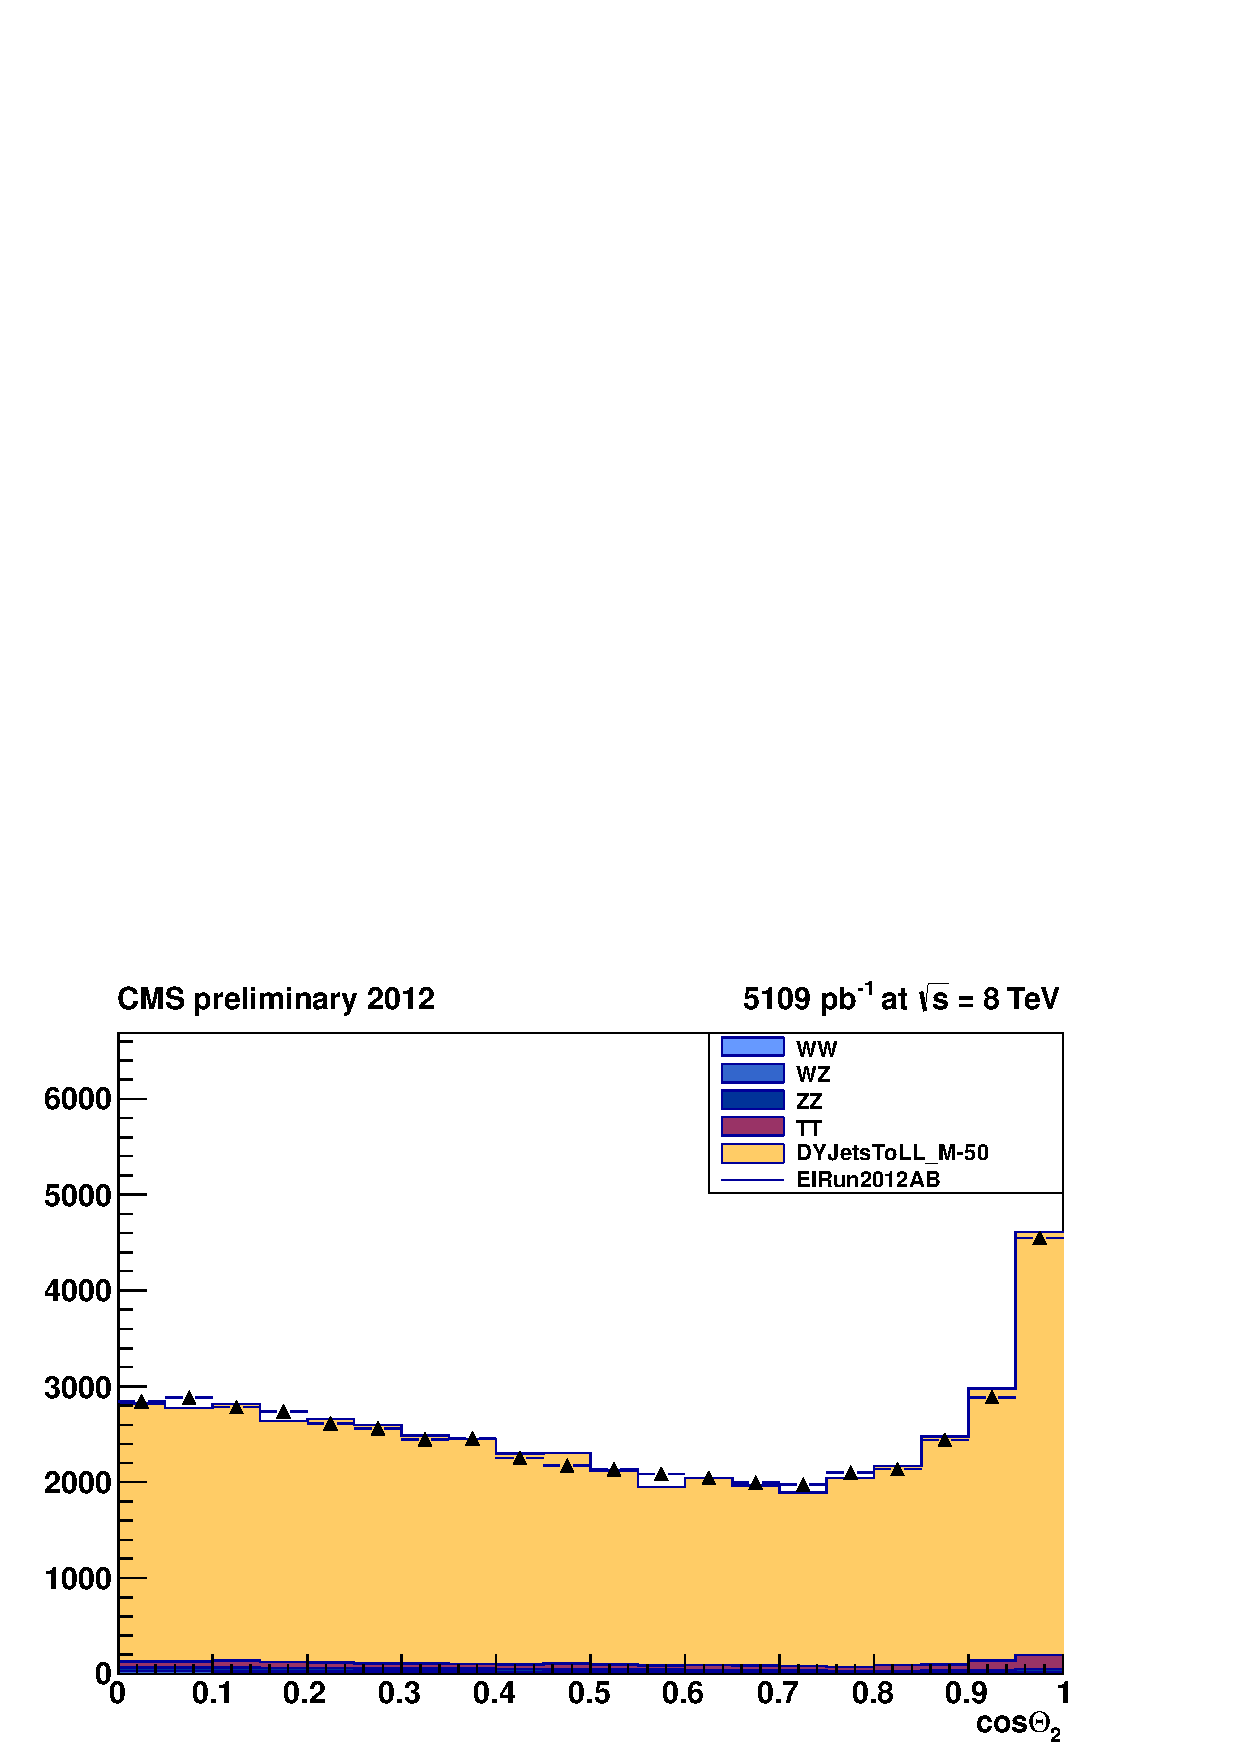
\includegraphics[width=0.33\textwidth]{images/plots/cosTheta2Refit_ElRun2012.png}
\includegraphics[width=0.33\textwidth]{images/plots/cosTheta1StarRefit_ElRun2012.png}
\\
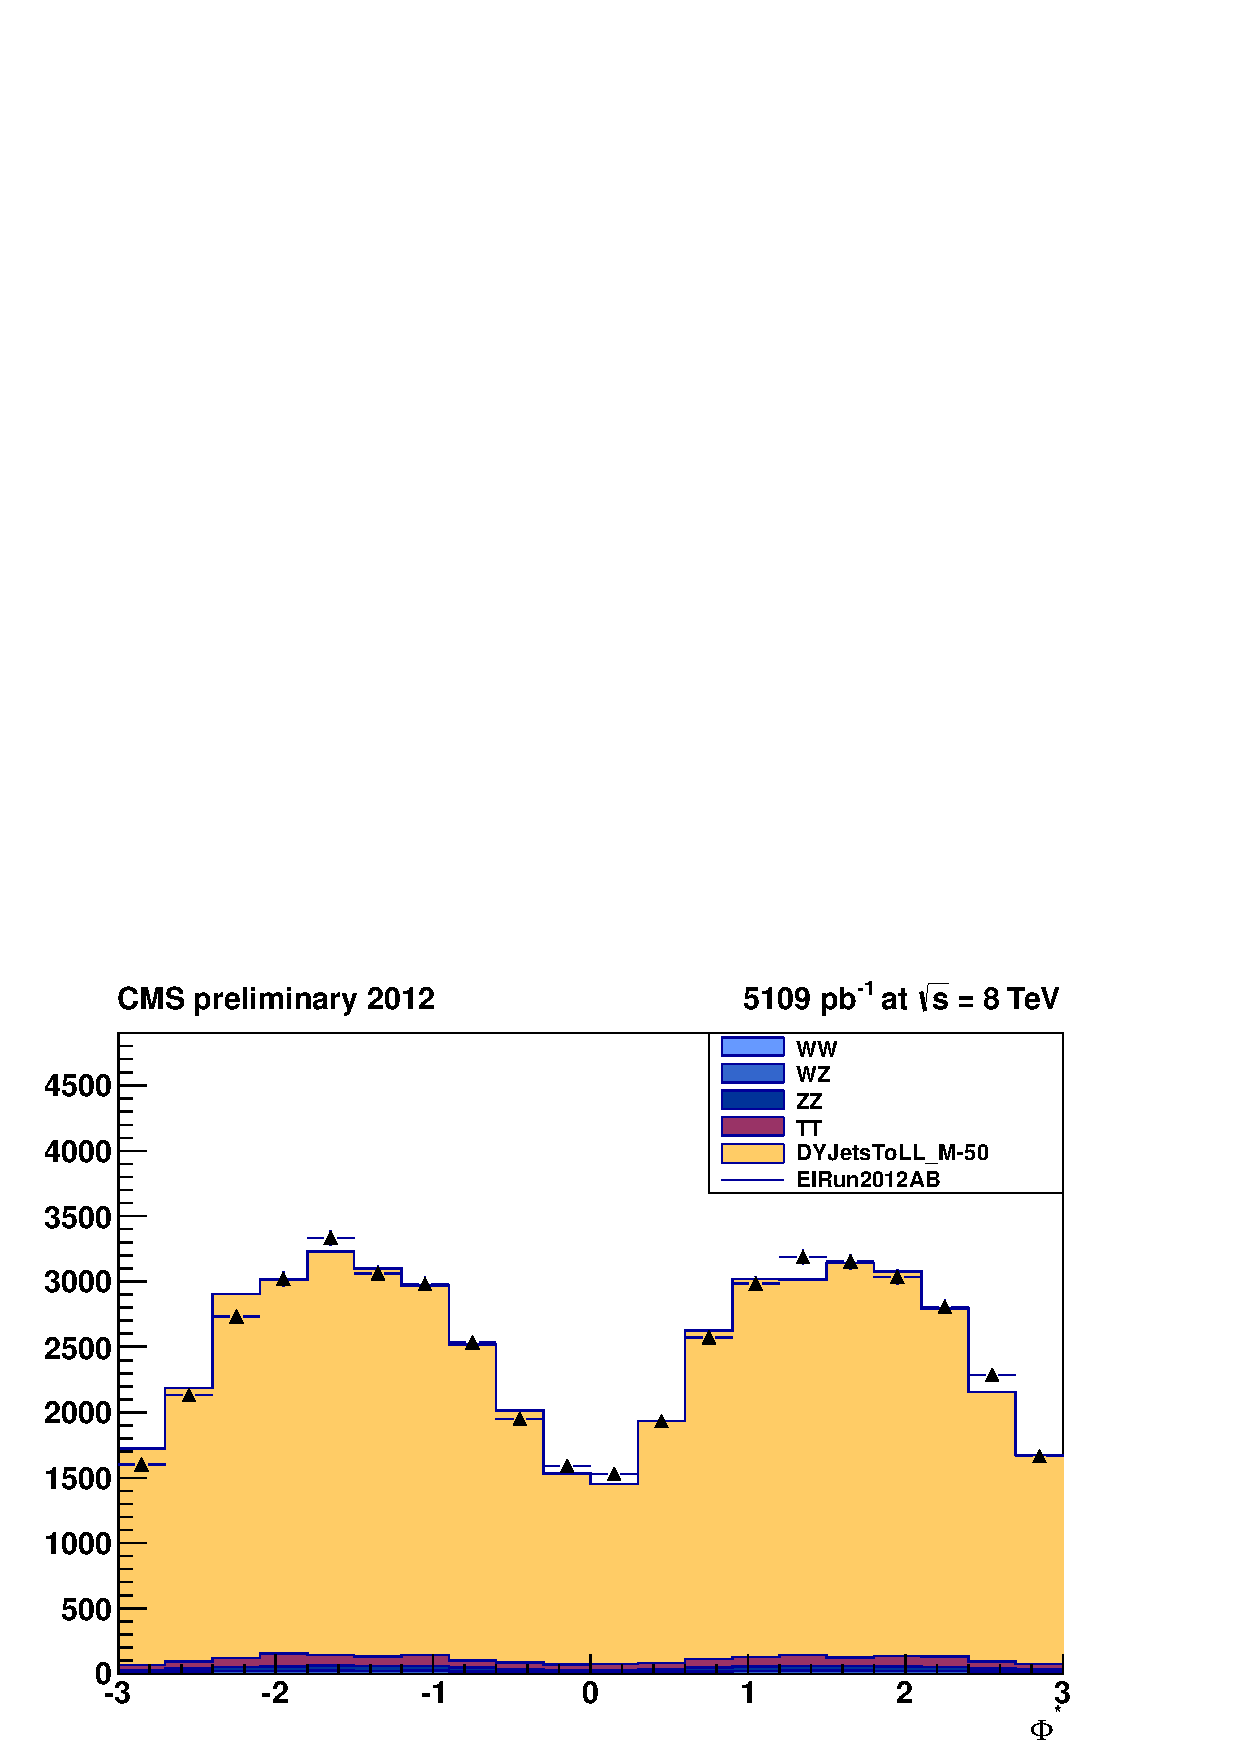
\includegraphics[width=0.33\textwidth]{images/plots/phiStarRefit_ElRun2012.png}
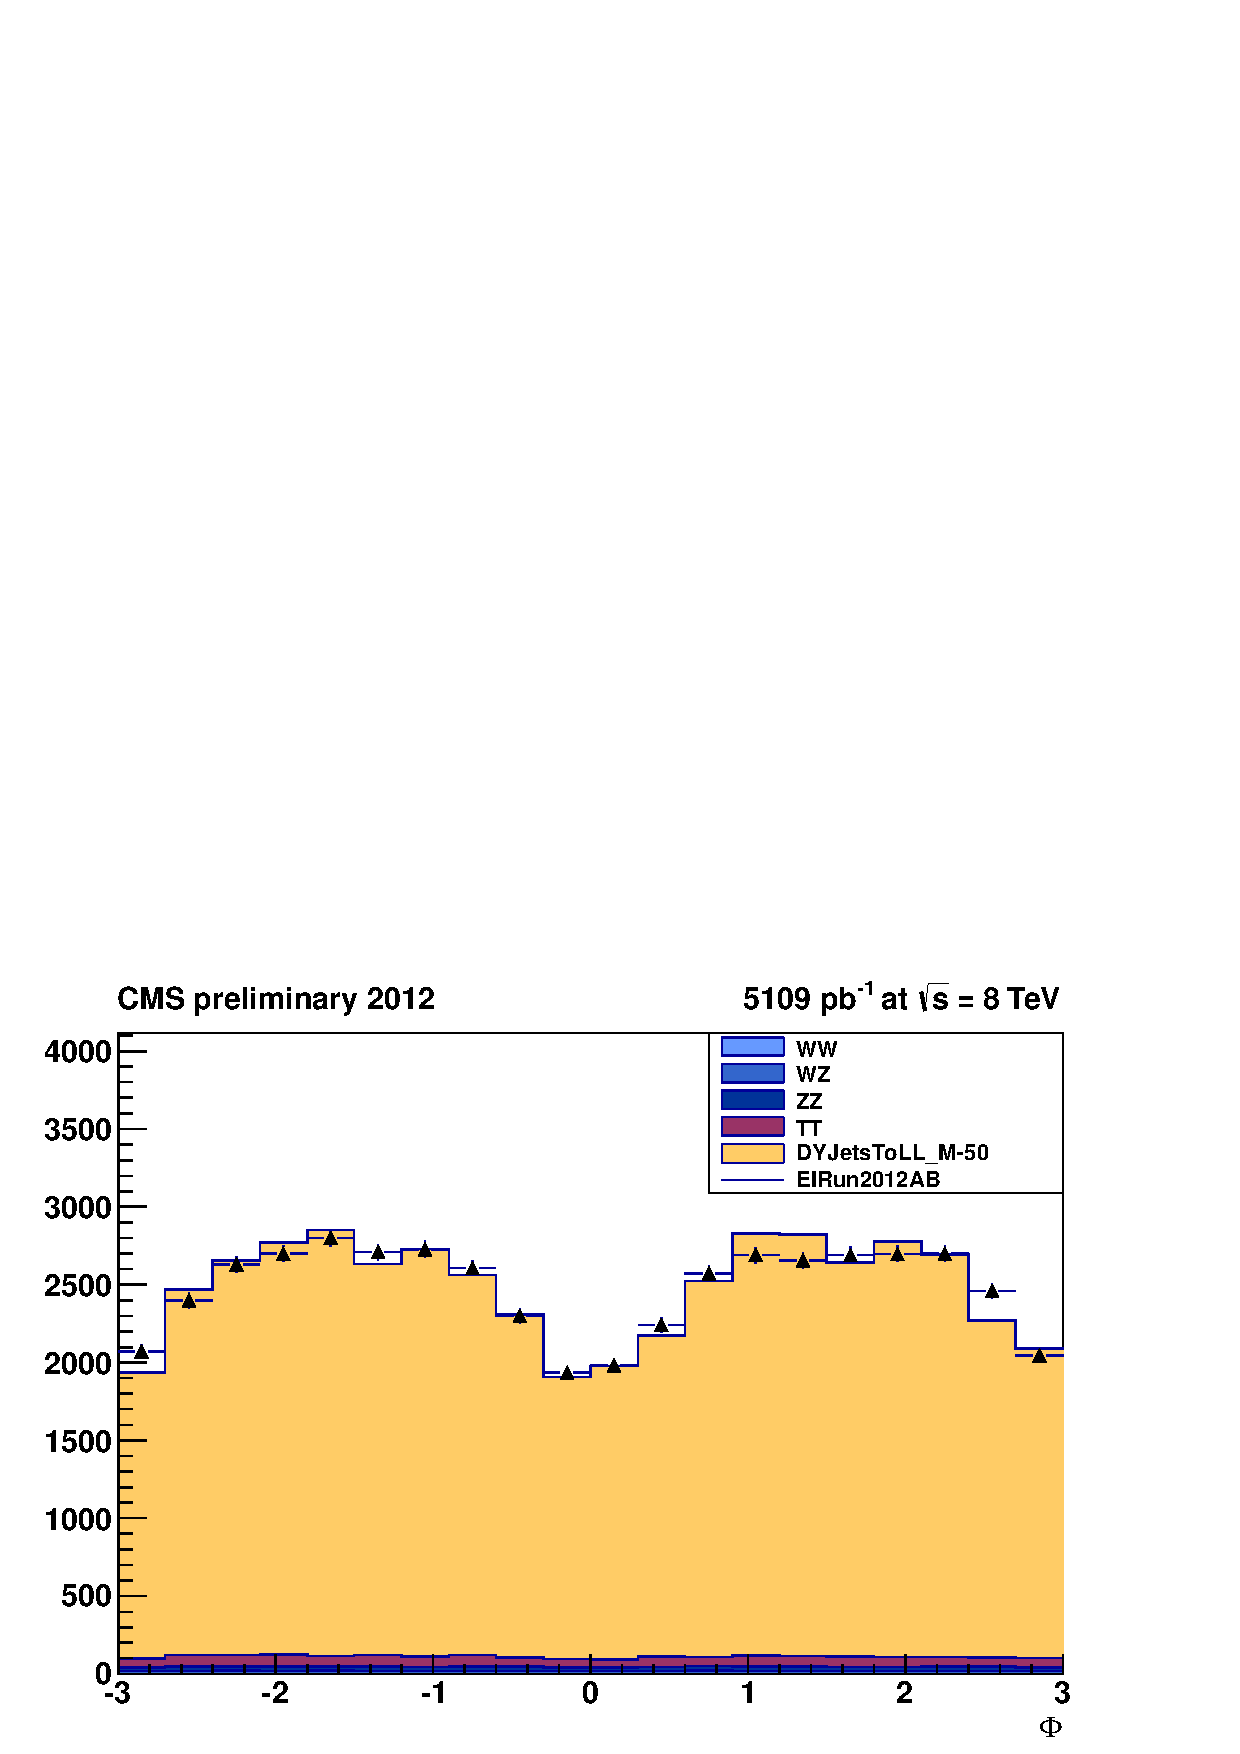
\includegraphics[width=0.33\textwidth]{images/plots/phiRefit_ElRun2012.png}
%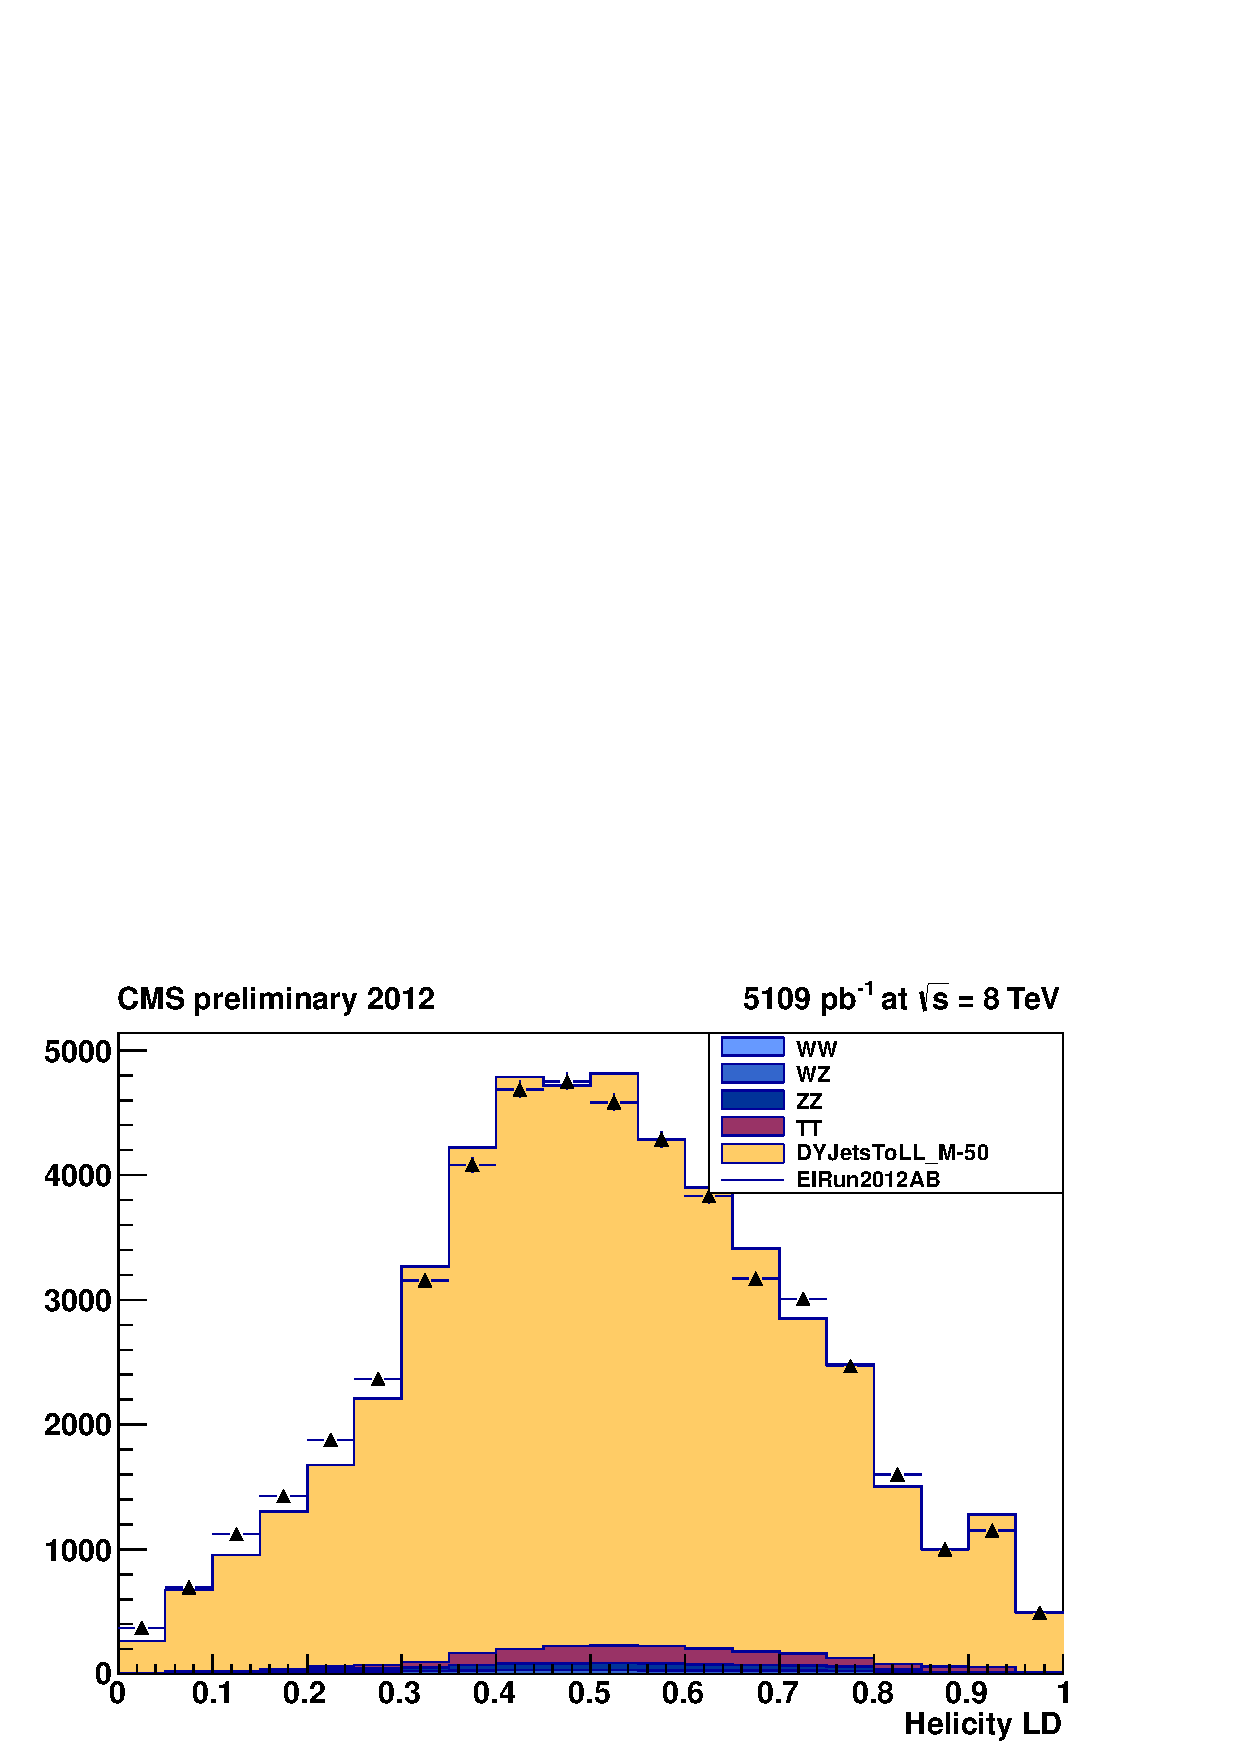
\includegraphics[width=0.33\textwidth]{images/plots/HelyLDRefit_ElRun2012.png}
\end{center}
\end{frame}


\begin{frame}{Muon Helicity and Production Angles}
\begin{center}
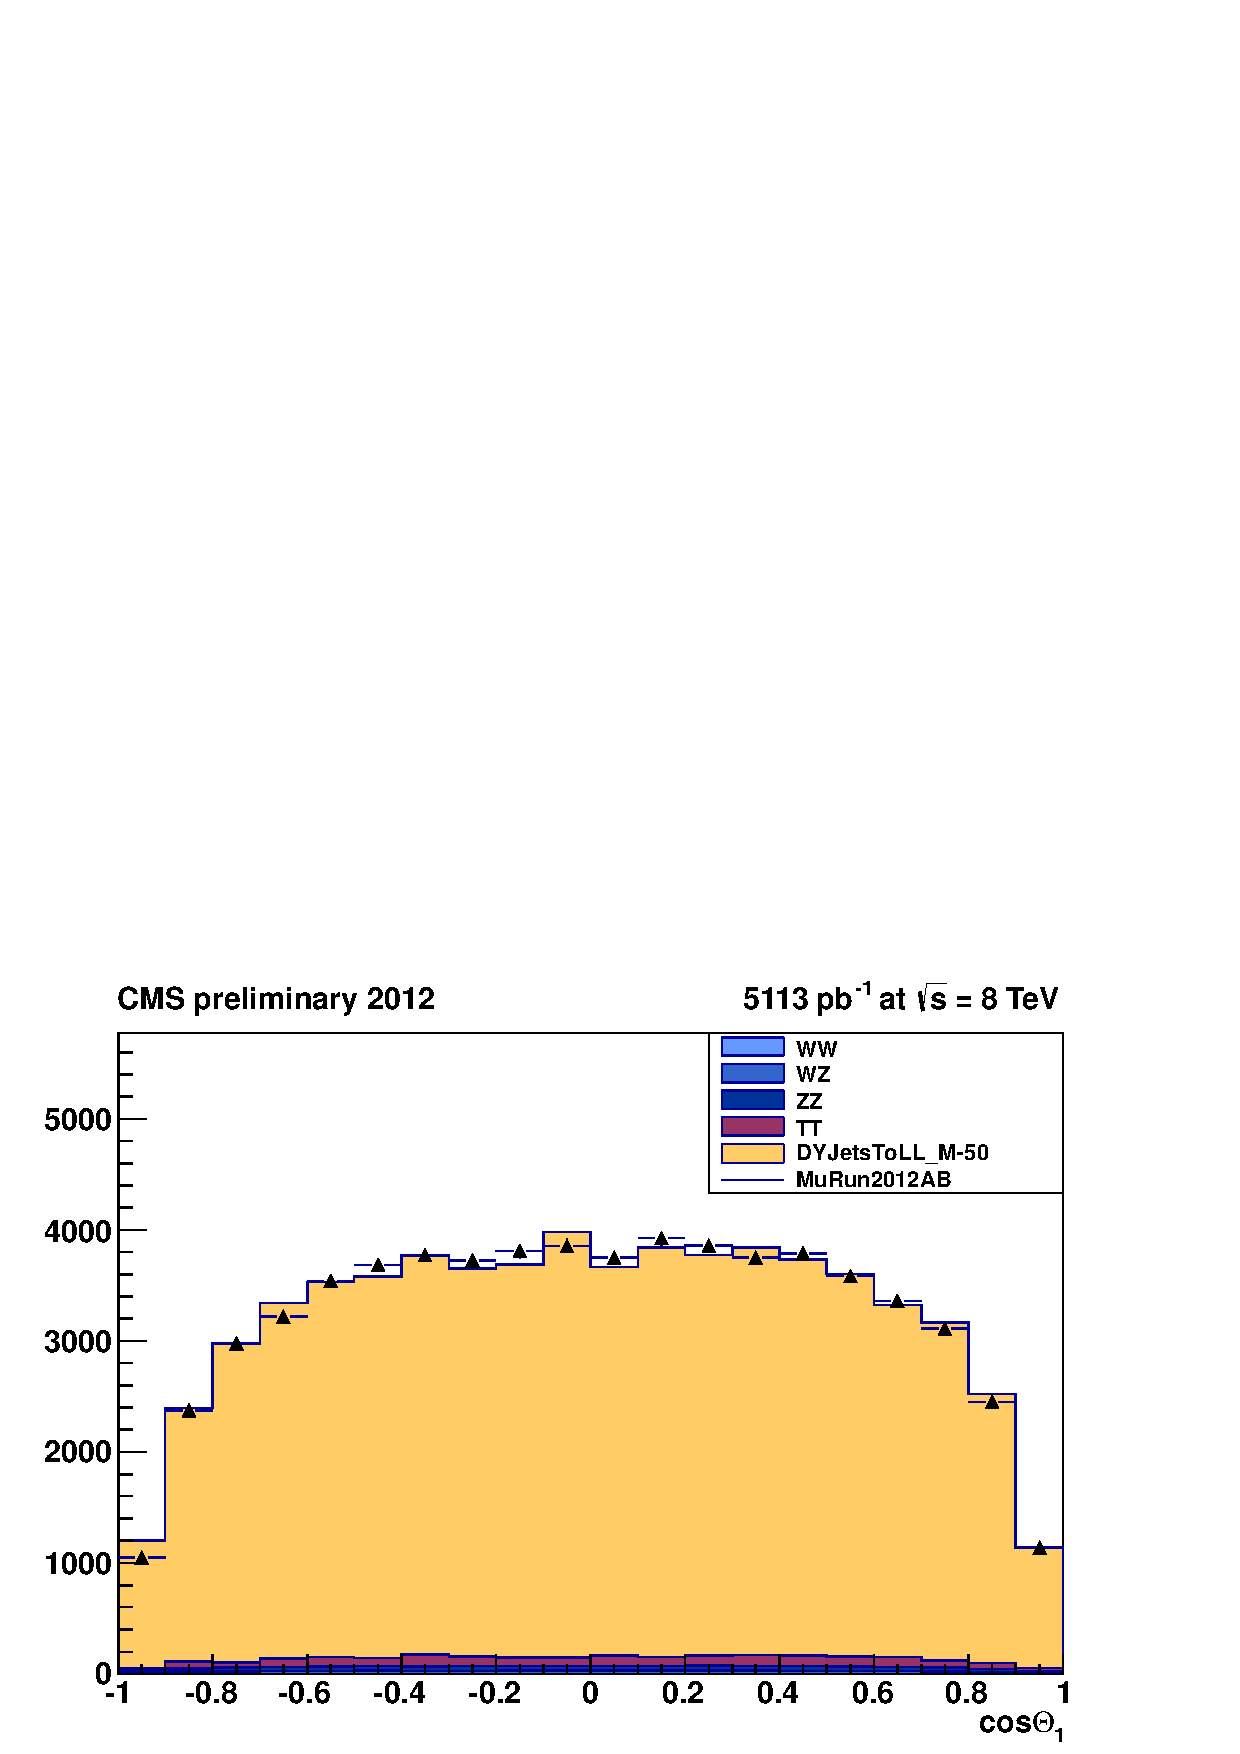
\includegraphics[width=0.33\textwidth]{images/plots/cosTheta1Refit_MuRun2012.png}
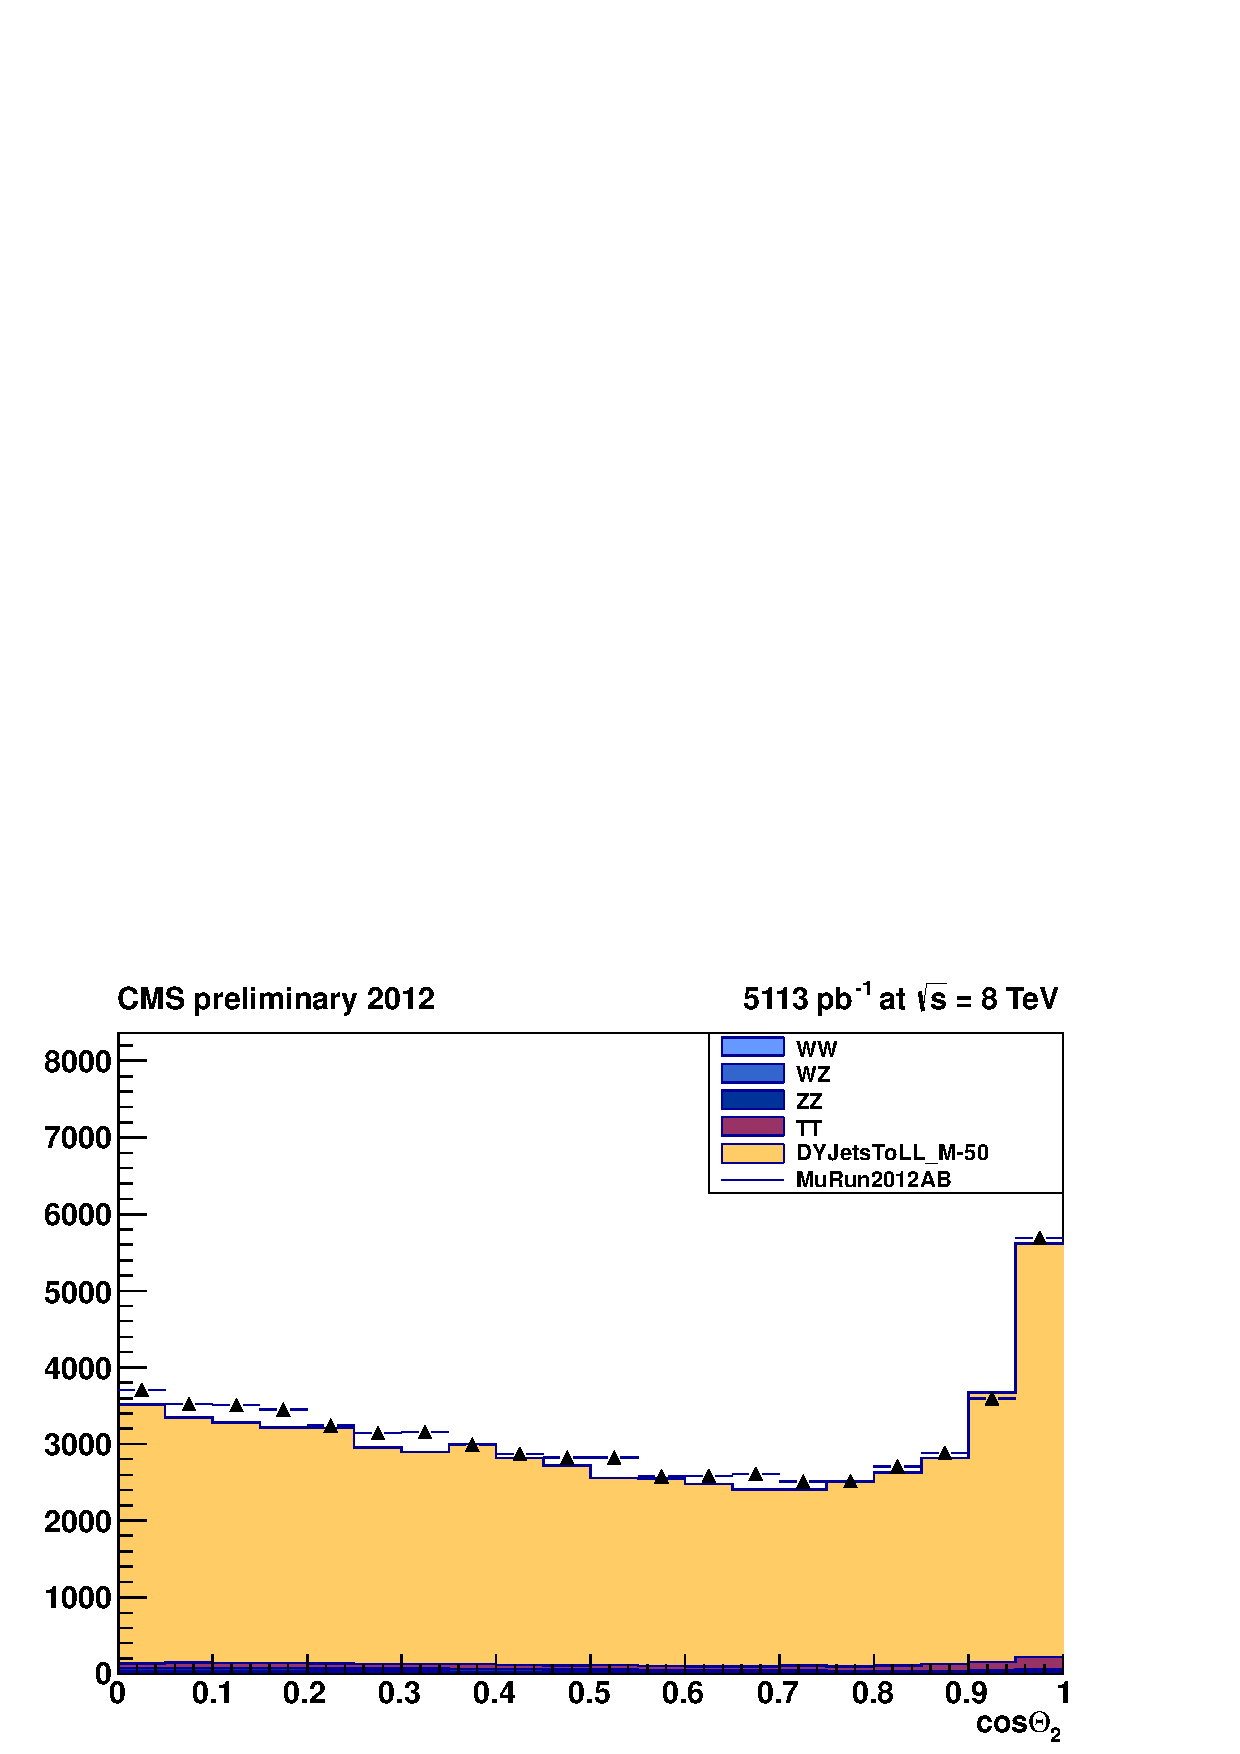
\includegraphics[width=0.33\textwidth]{images/plots/cosTheta2Refit_MuRun2012.png}
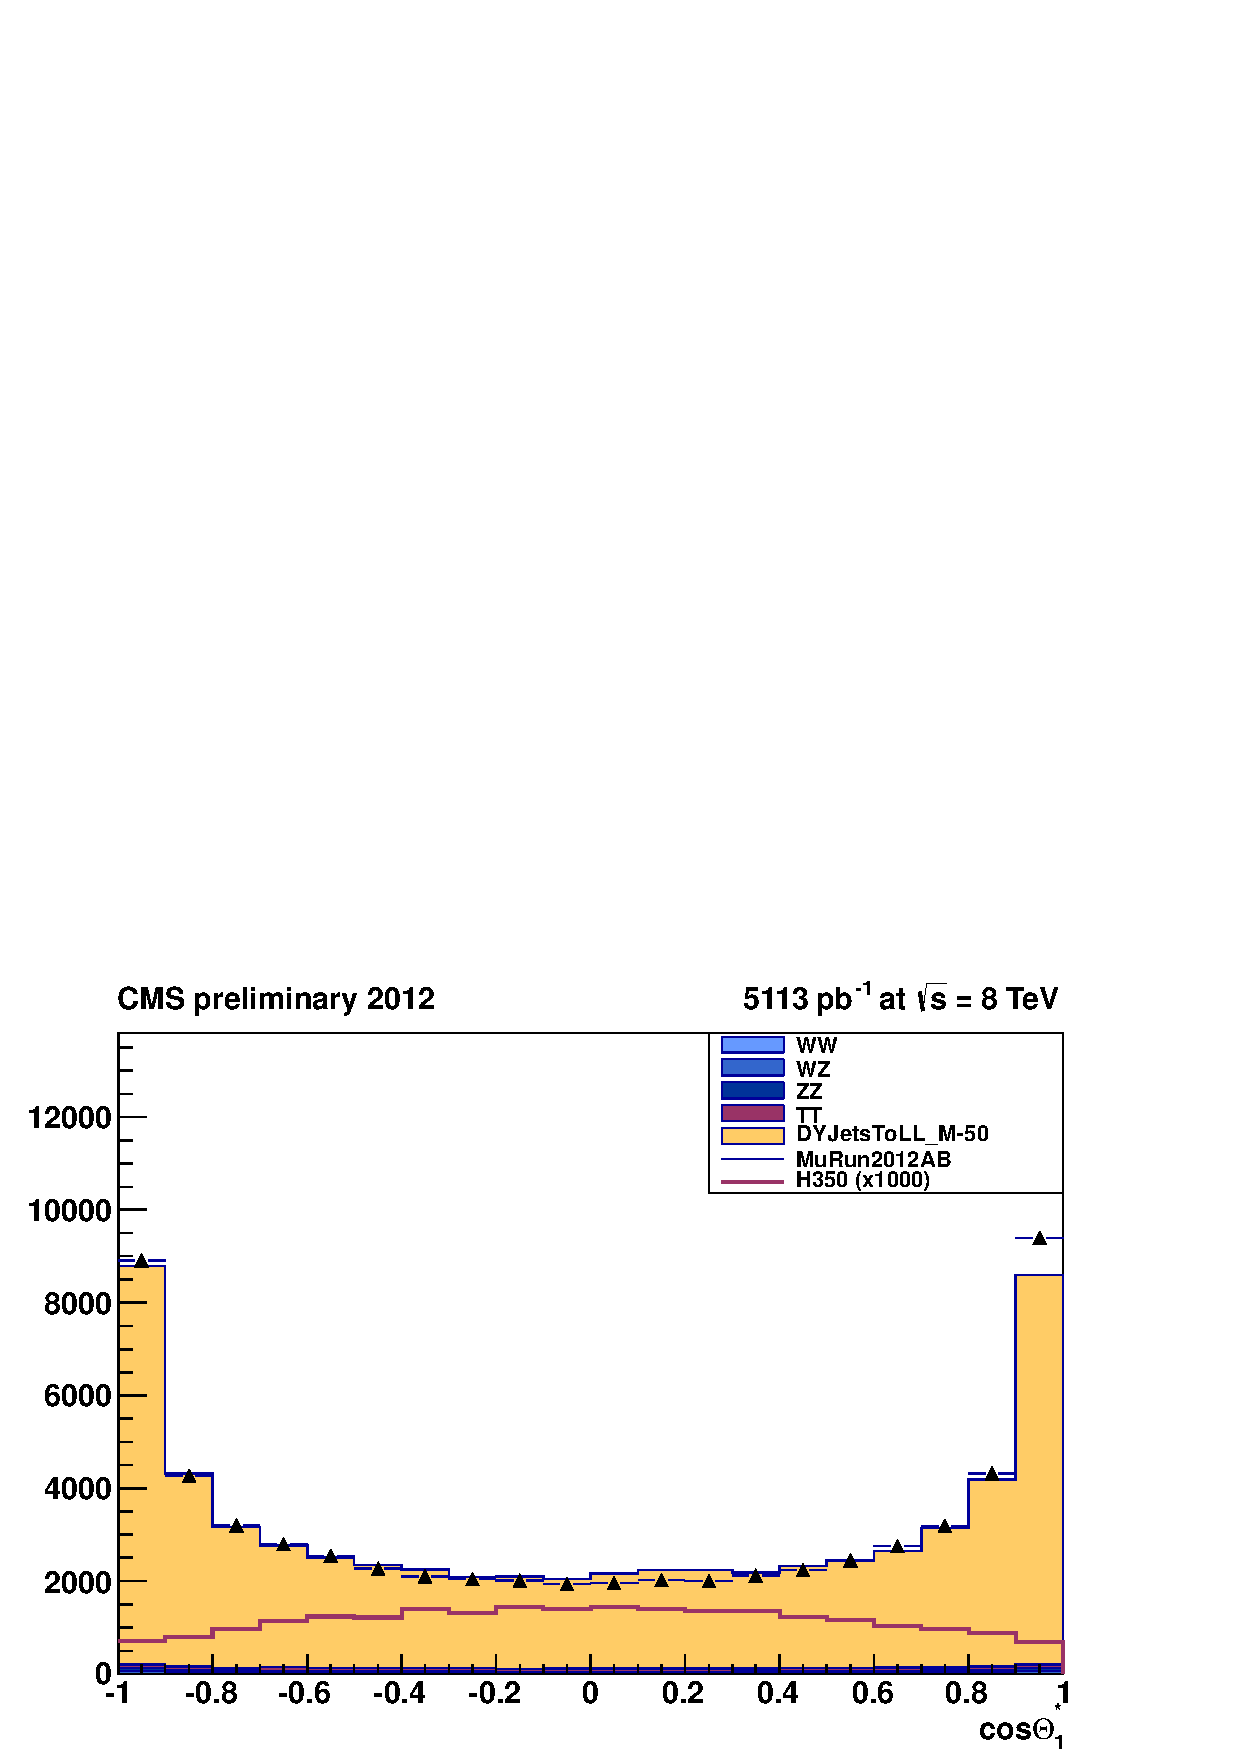
\includegraphics[width=0.33\textwidth]{images/plots/cosTheta1StarRefit_MuRun2012.png}
\\
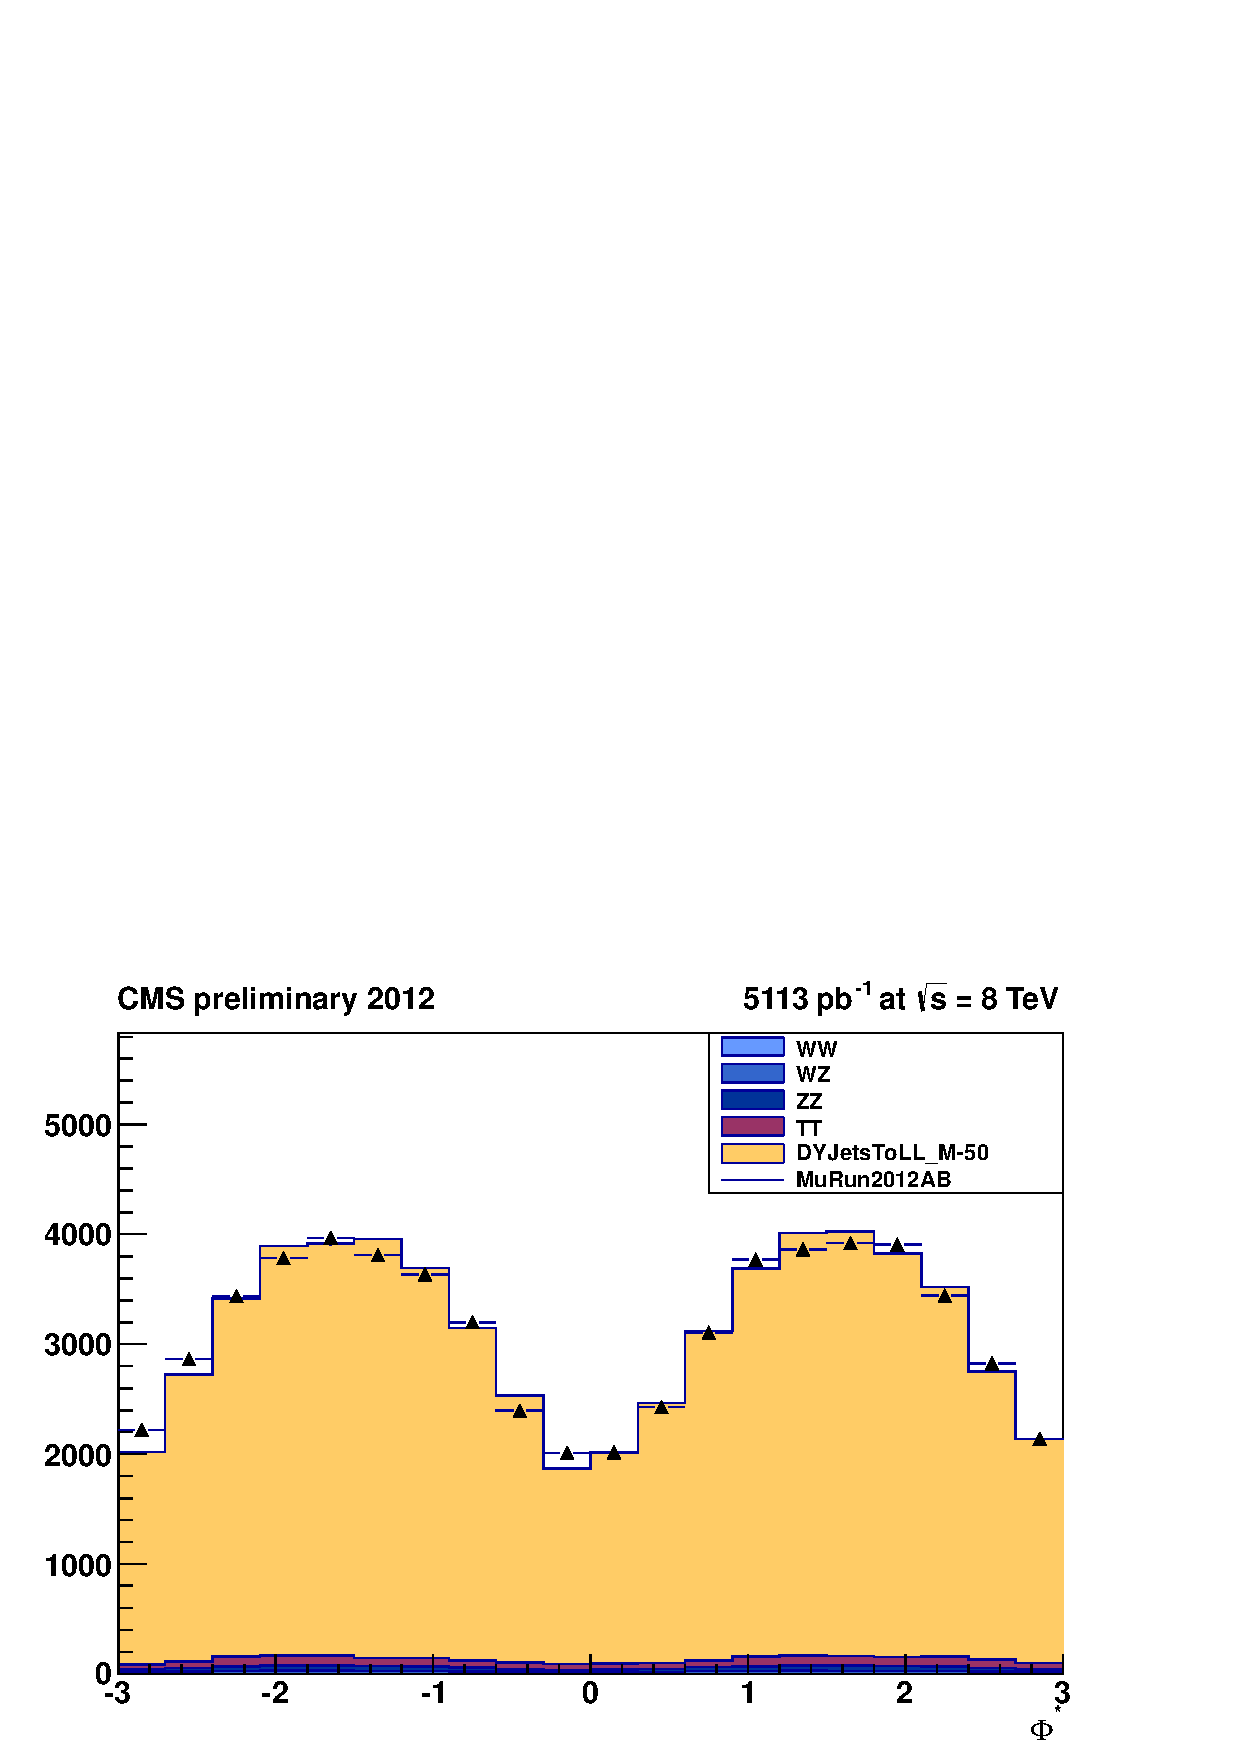
\includegraphics[width=0.33\textwidth]{images/plots/phiStarRefit_MuRun2012.png}
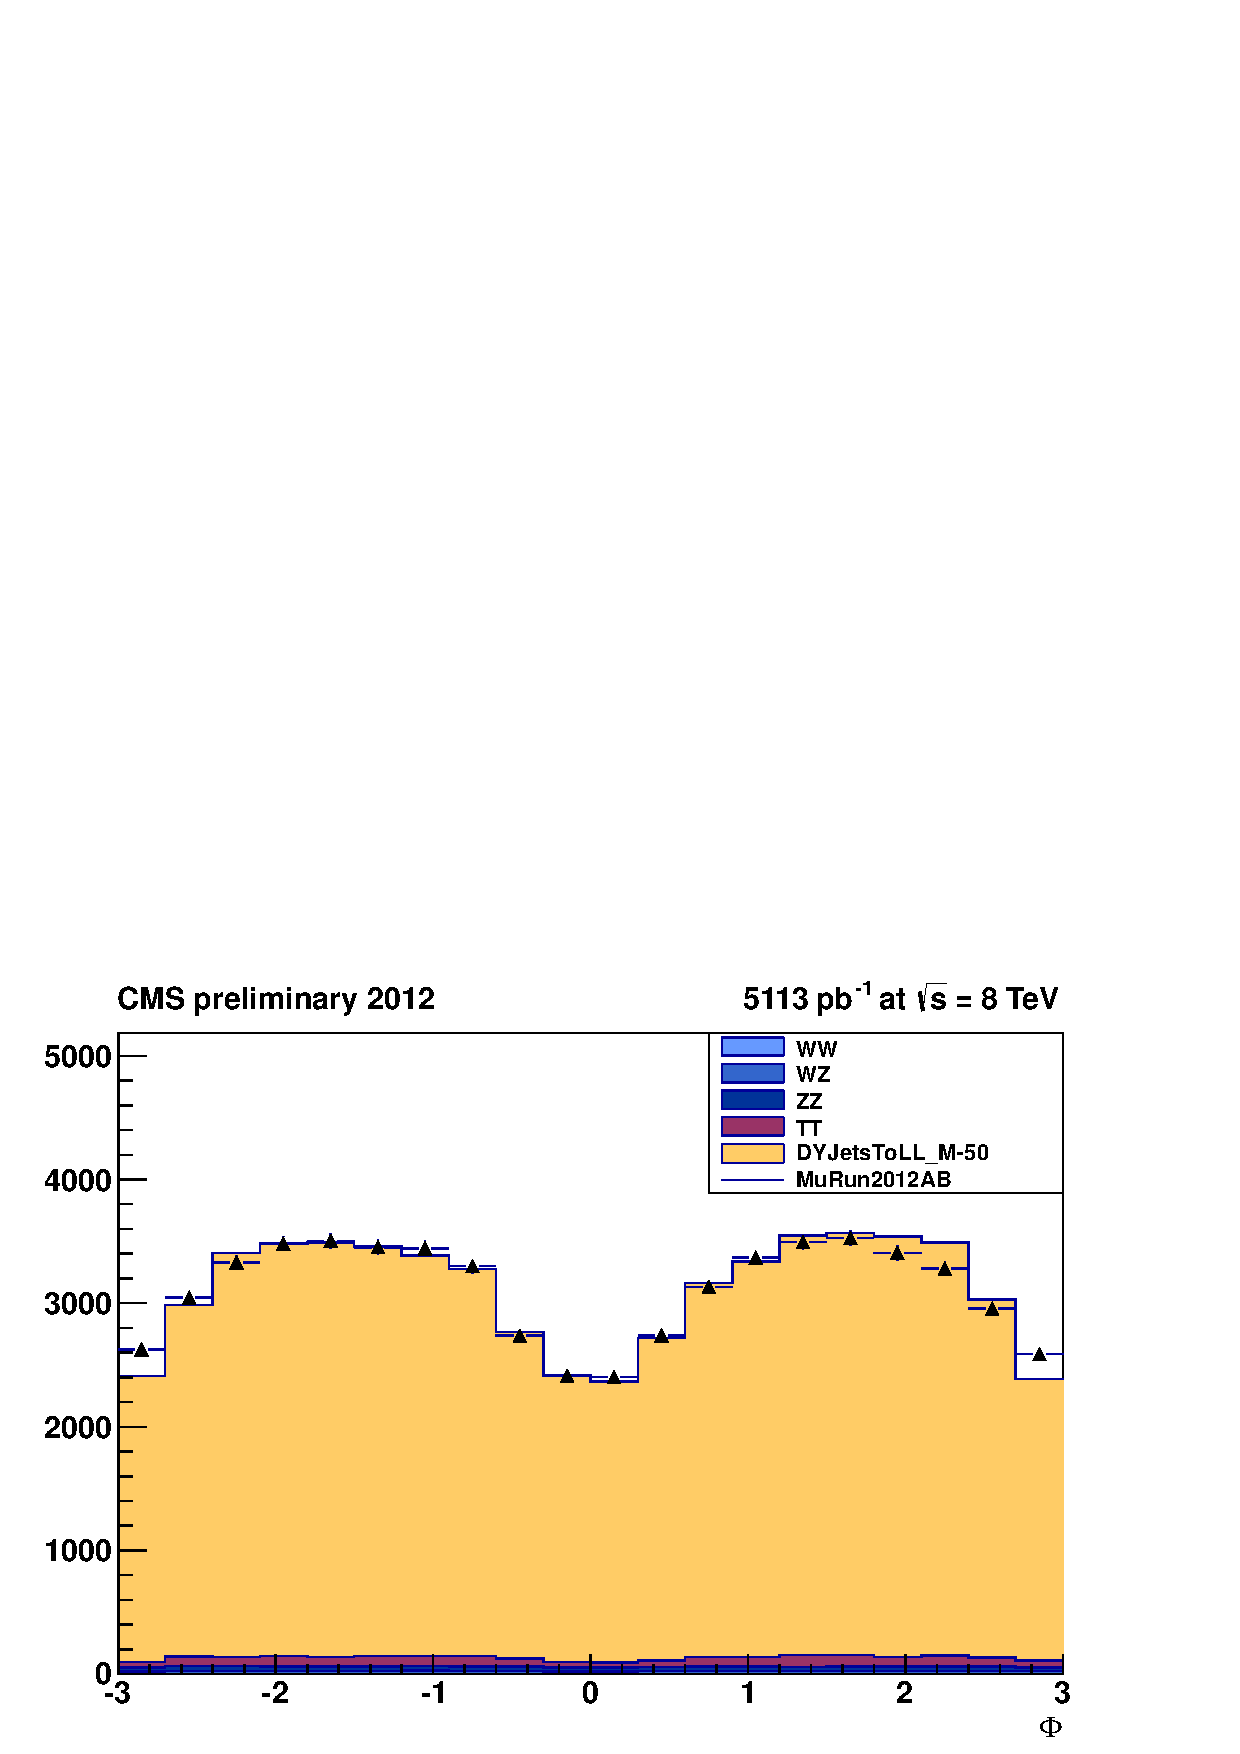
\includegraphics[width=0.33\textwidth]{images/plots/phiRefit_MuRun2012.png}

\end{center}
\end{frame}



\begin{frame}{Angular Distribution Fits}
\begin{center}
Example fits at for 500 GeV (475 - 550 GeV).
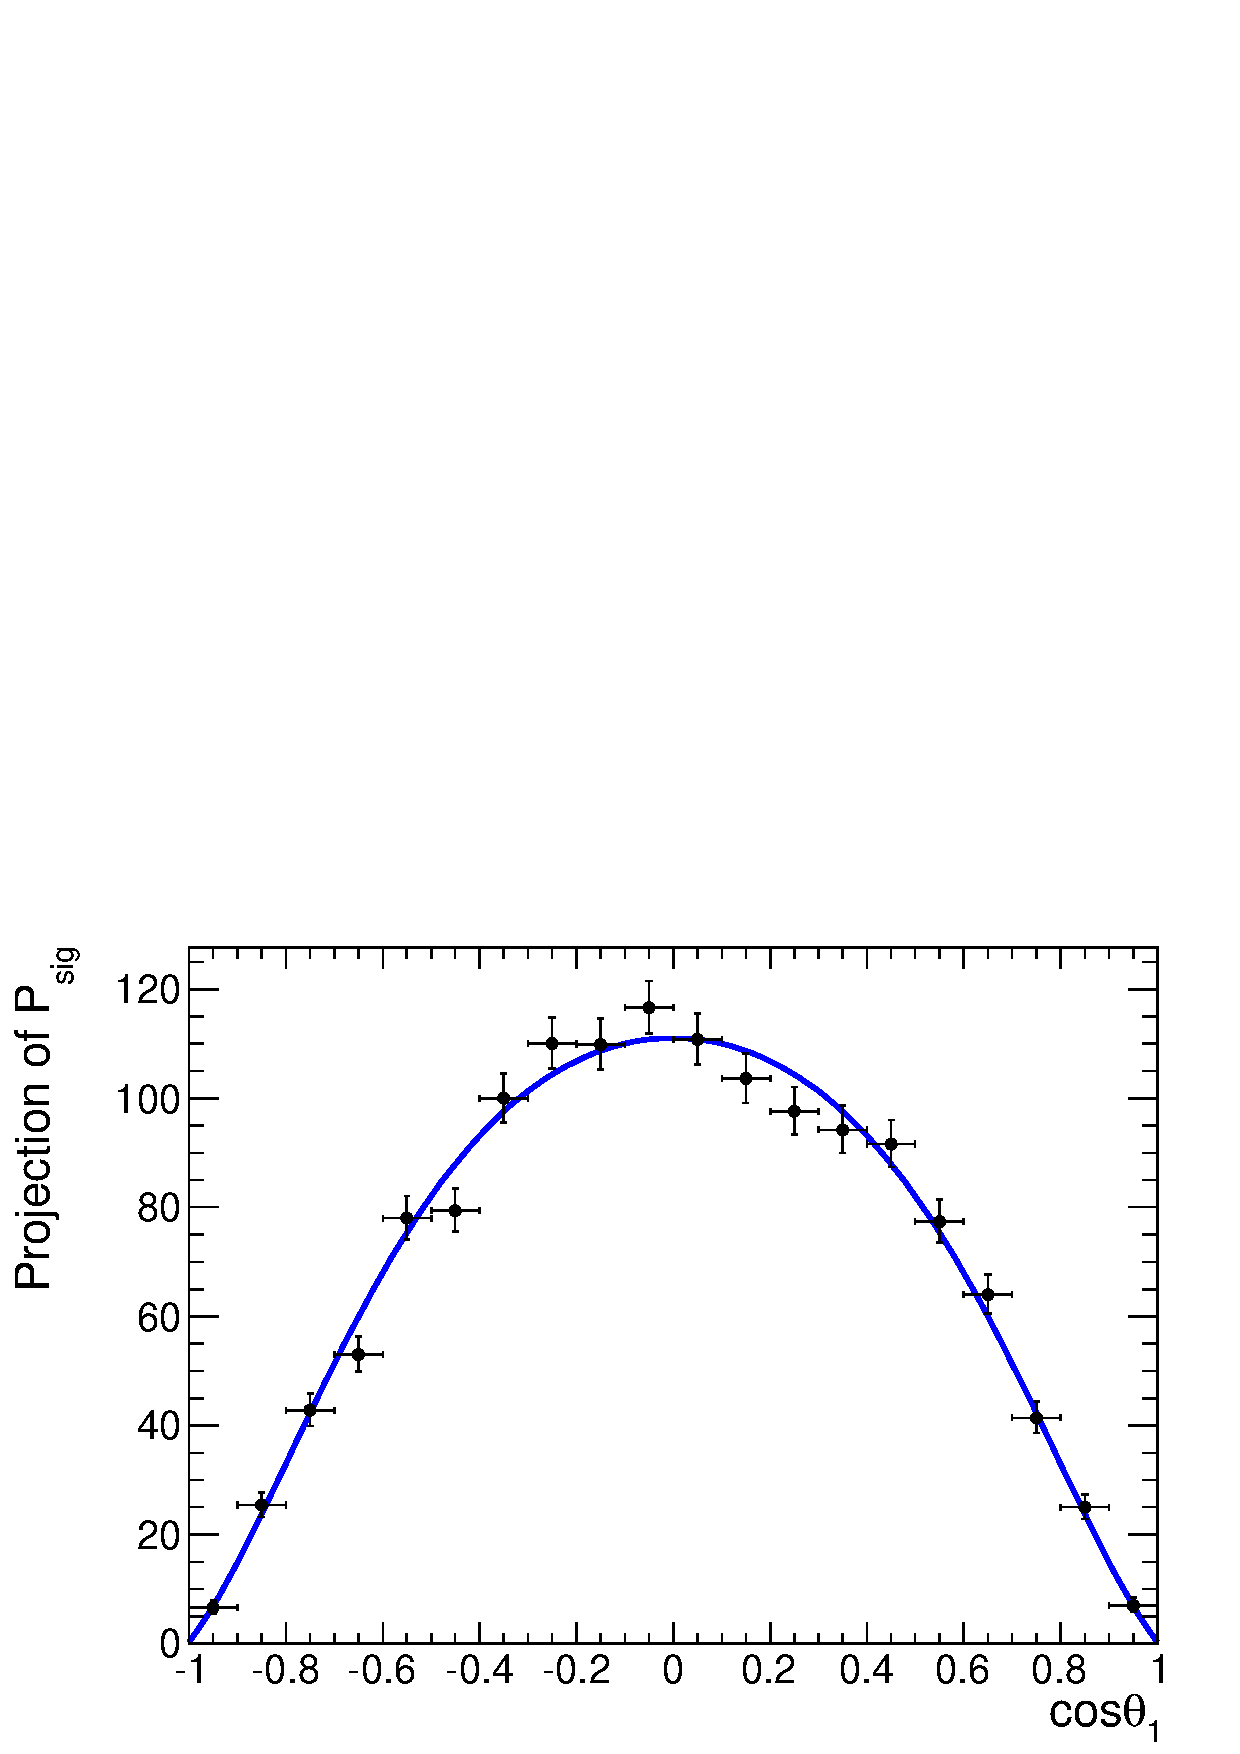
\includegraphics[width=0.33\textwidth]{images/plots/sigPDF_CosTheta1proj_500.pdf}
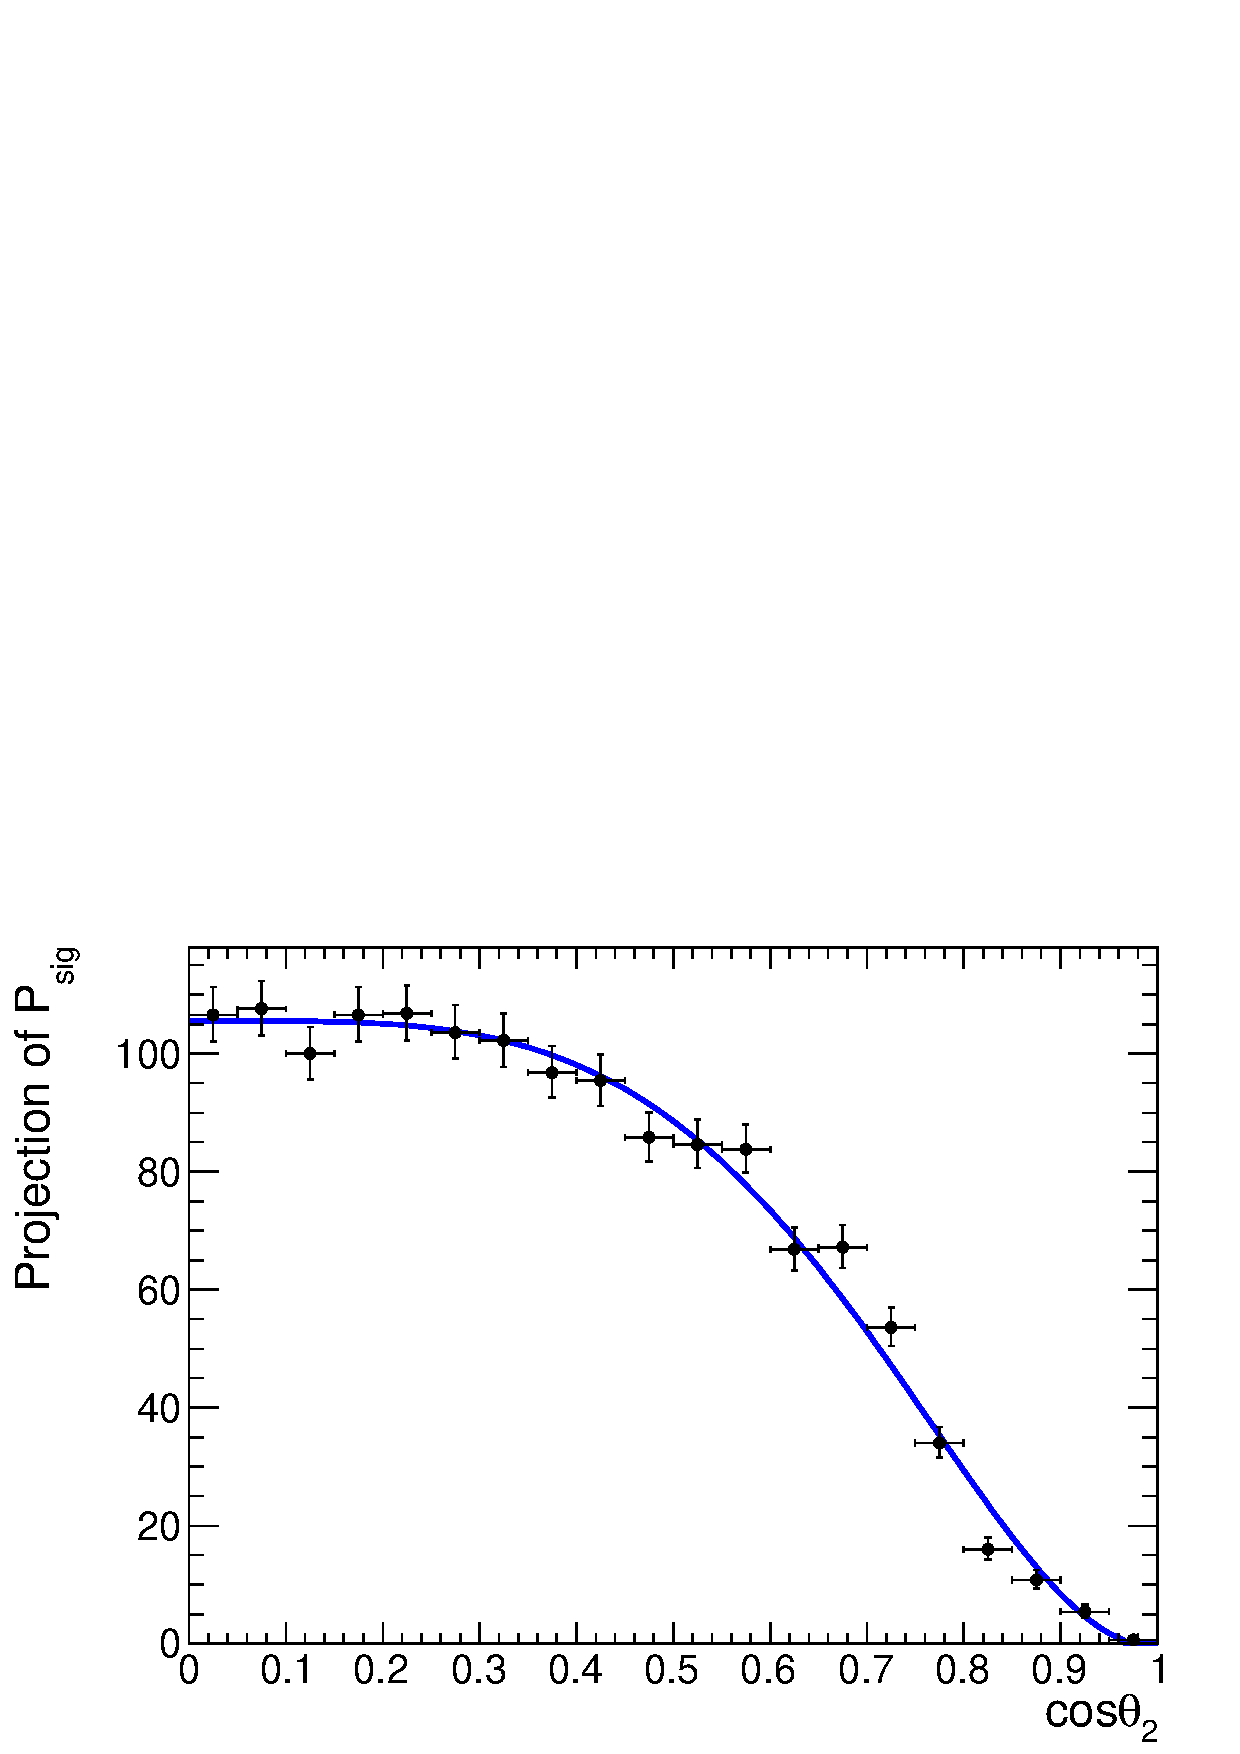
\includegraphics[width=0.33\textwidth]{images/plots/sigPDF_CosTheta2proj_500.pdf}
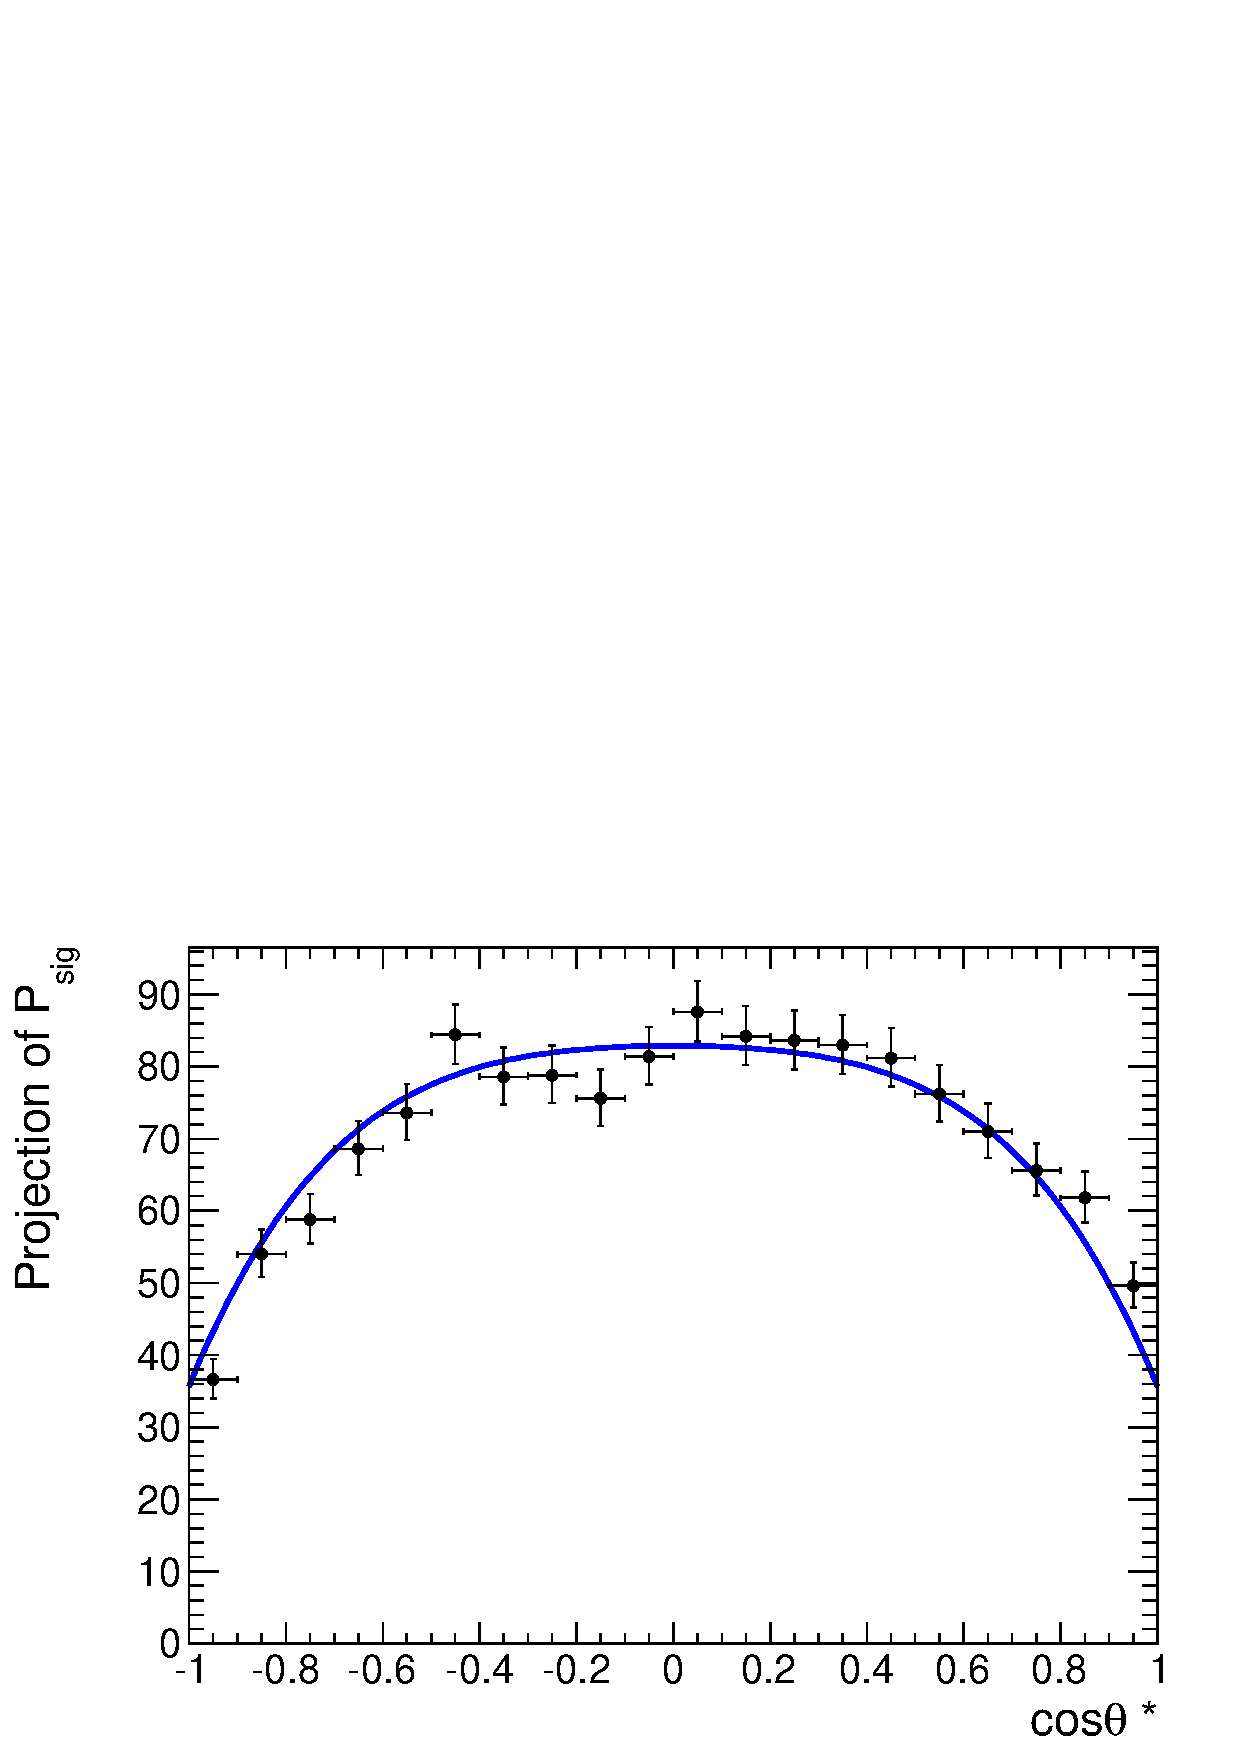
\includegraphics[width=0.33\textwidth]{images/plots/sigPDF_CosThetaSproj_500.pdf}
\\
\includegraphics[width=0.33\textwidth]{images/plots/sigPDF_Phiproj_500.pdf}
\includegraphics[width=0.33\textwidth]{images/plots/sigPDF_PhiStar1proj_500.pdf}

%sigPDF_CosTheta1proj_500.pdf  sigPDF_CosTheta2proj_500.pdf  sigPDF_CosThetaSproj_500.pdf  sigPDF_Phiproj_500.pdf  sigPDF_PhiStar1proj_500.pdf

\end{center}
\end{frame}



\begin{frame}{Helicity LD}
\begin{center}
$LD = \dfrac{P_{sig}}{P_{sig} + P_{bkg}}$
\\
%\vpace{1em}
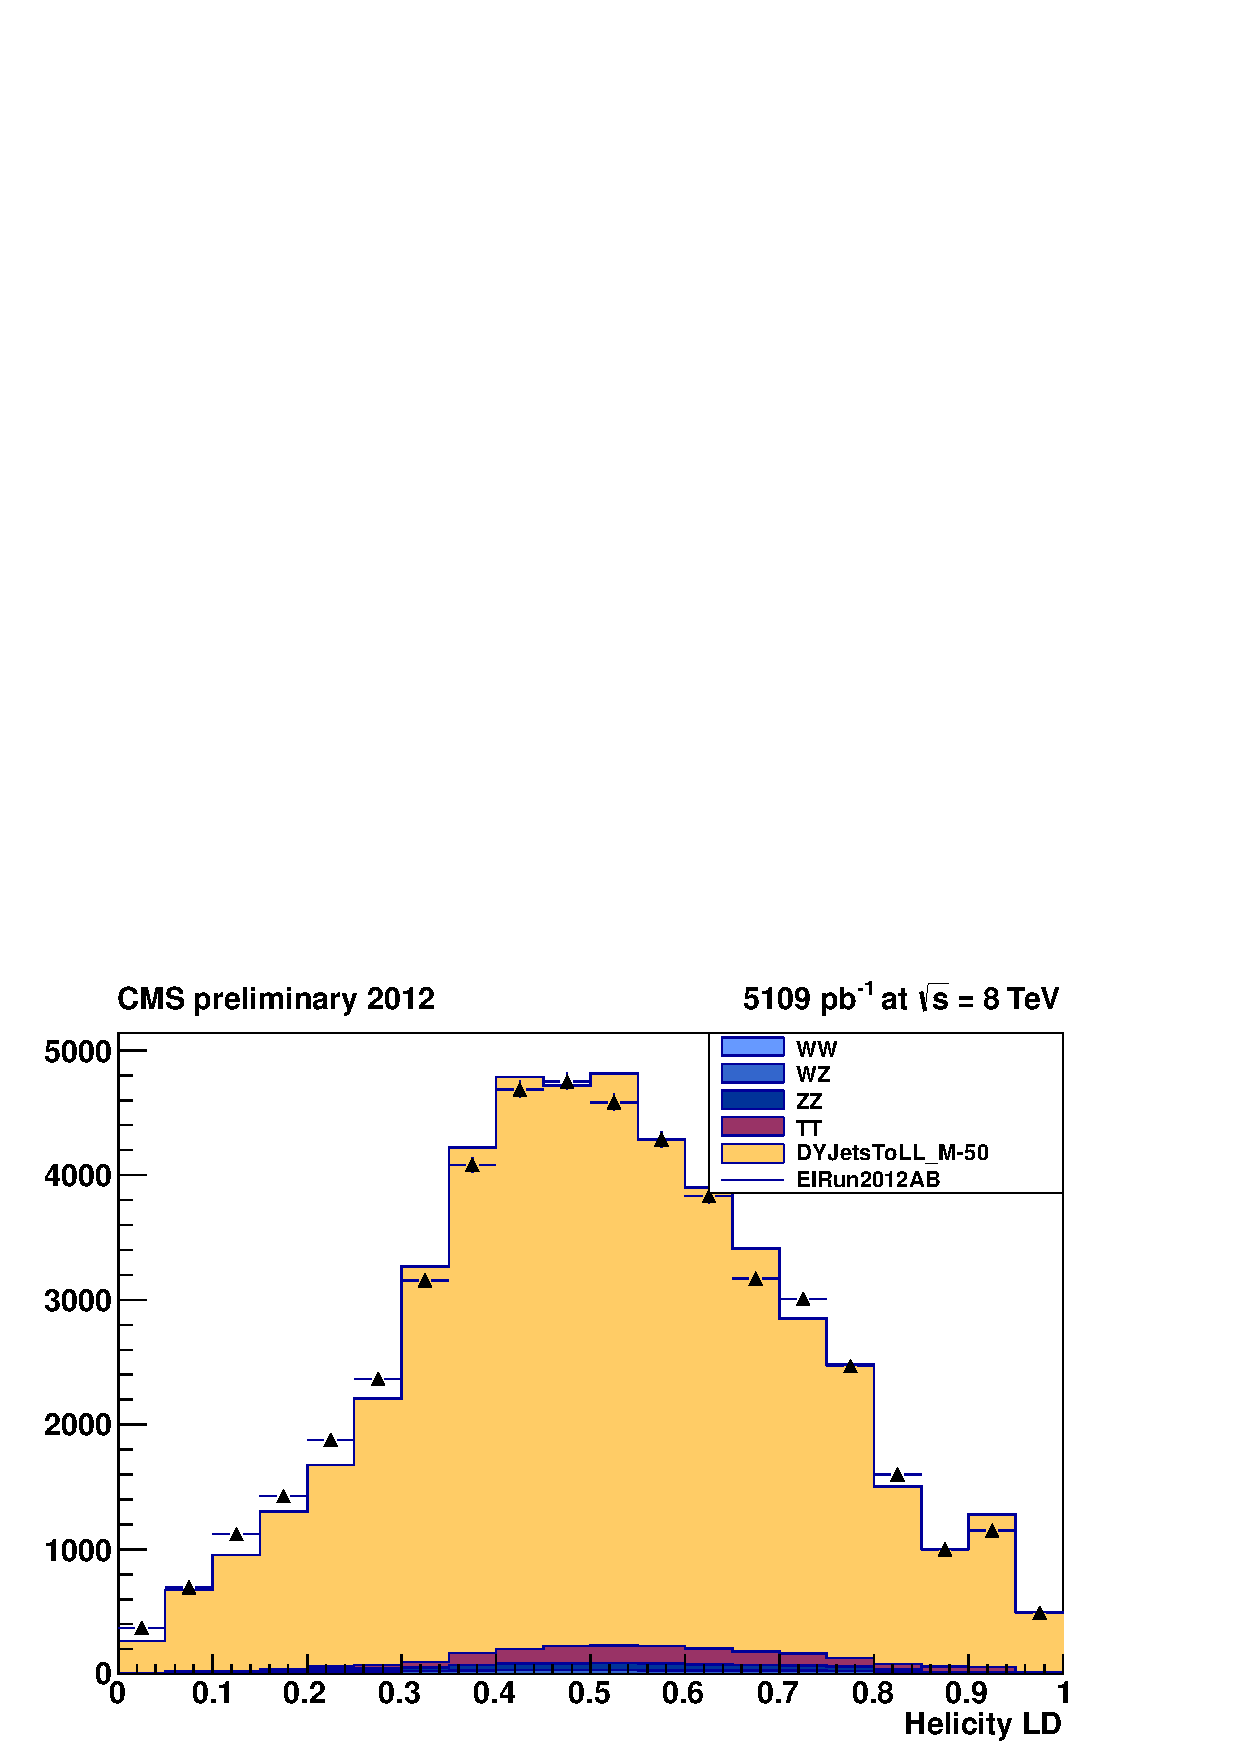
\includegraphics[width=0.5\textwidth]{images/plots/HelyLDRefit_ElRun2012.png}
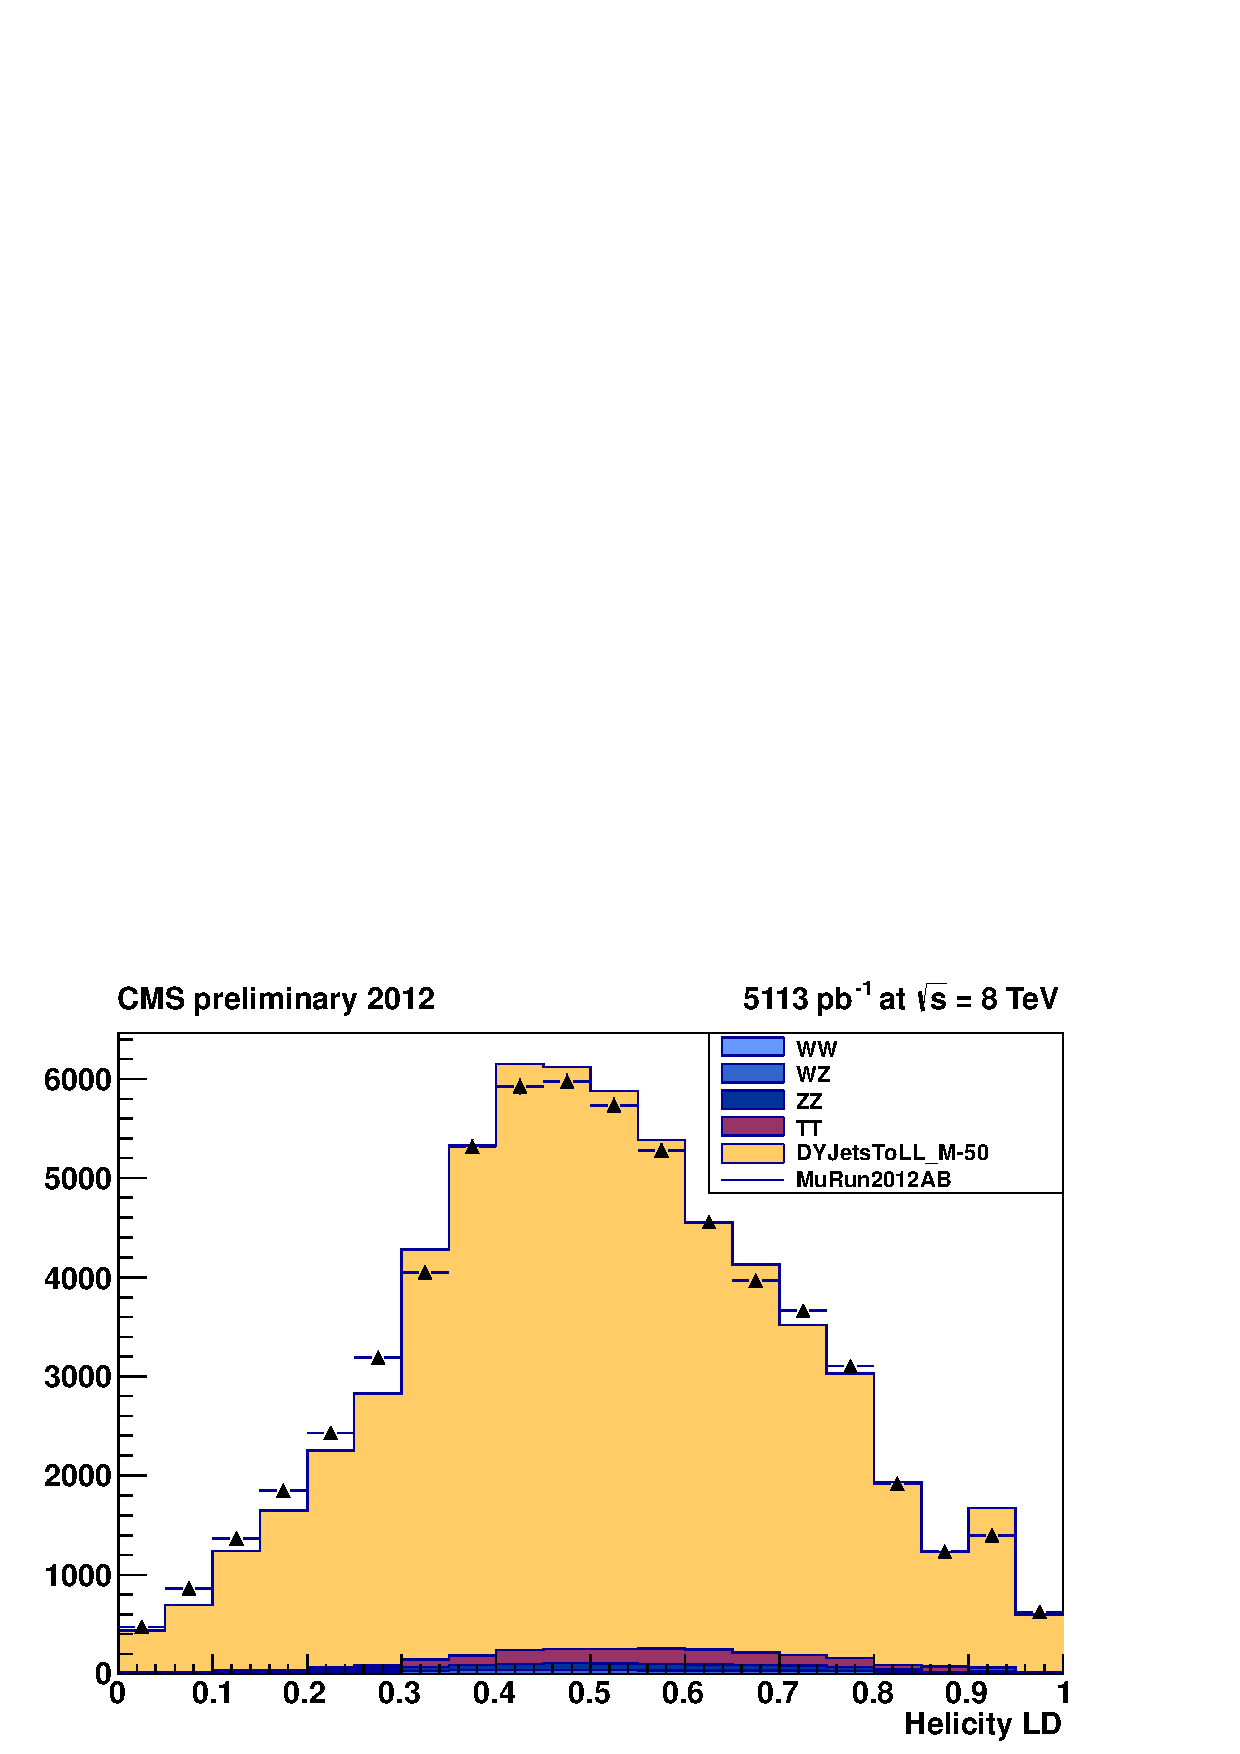
\includegraphics[width=0.5\textwidth]{images/plots/HelyLDRefit_MuRun2012.png}
\\
\vspace{2em}
\tiny
\begin{tabular}{|l|c|c|c|}
\hline
 & 0 $b$-tag & 1 $b$-tag  & 2 $b$-tag \\
\hline
Helicity LD &  $>(0.55+0.00025\times m_{ZZ})$ & $>(0.302+0.000656\times m_{ZZ})$ & $> 0.5$ \\
%\vspace{-0.2cm}
%Quark-Gluon LD &  $>0.10$ & -- & --  \\
%\vspace{-0.2cm}
%\vspace{-0.2cm}
\hline
\end{tabular}
\end{center}
\end{frame}



\begin{frame}{Neural Network with TMVA Package}
\begin{center}
\includegraphics[width=0.8\linewidth]{images/plots/NN/nn_network_architecture}
\end{center}
\end{frame}



\begin{frame}{Neural Network Training and Testing}
\begin{center}
The trainings are done after preselection and additionally require at least one B-tagged Medium jet Left: Training 400 GeV Higgs boson with a MLP neural network.  Right: Training 400 GeV Higgs boson with a Likelihood.
\includegraphics[width=0.5\linewidth]{images/plots/NN/MLP_TCHEM.pdf}
\includegraphics[width=0.5\linewidth]{images/plots/NN/Likelihood_TCHEM.pdf}
\end{center}
\end{frame}


\begin{frame}{MLP vs Helicity LD}
\begin{center}
The working point is the background rejection point that we currently achieve in the two tag region in our analysis.
\includegraphics[width=0.7\linewidth]{images/plots/NN/pretag_ROC_wincut.pdf}
\end{center}
\end{frame}


\begin{frame}{High Mass MVA Introduction}
\begin{itemize}
\item
  Since the current helyLD optimization does not work at high mass I am looking at the performance of the straight forward MLP neural network performance in the High Mass region.
\item
  This looks at a training on the Higgs 400GeV signal sample (a trianing that works well for 300-600 as shown in previous talks) as well as the same training but on a Higgs 800 GeV signal sample.
\item
  These signal samples are the Gluon-Gluon samples
\end{itemize}
\end{frame}

%\begin{frame}{Optimization}
%\begin{itemize}
%  \item
%    Look at High Higgs mass (600,700,800,900,1000 GeV)
%  \item
%    Trained on 5 angular variables with signal of 400
%  \item
%    Previously shown similar results of helyLD with MLP NN for lower mass range (300,400,500,600)
%\end{itemize}
%\begin{center}
%Preselection    \hspace{7em}           Preselction + Higgs 400 mass cut
%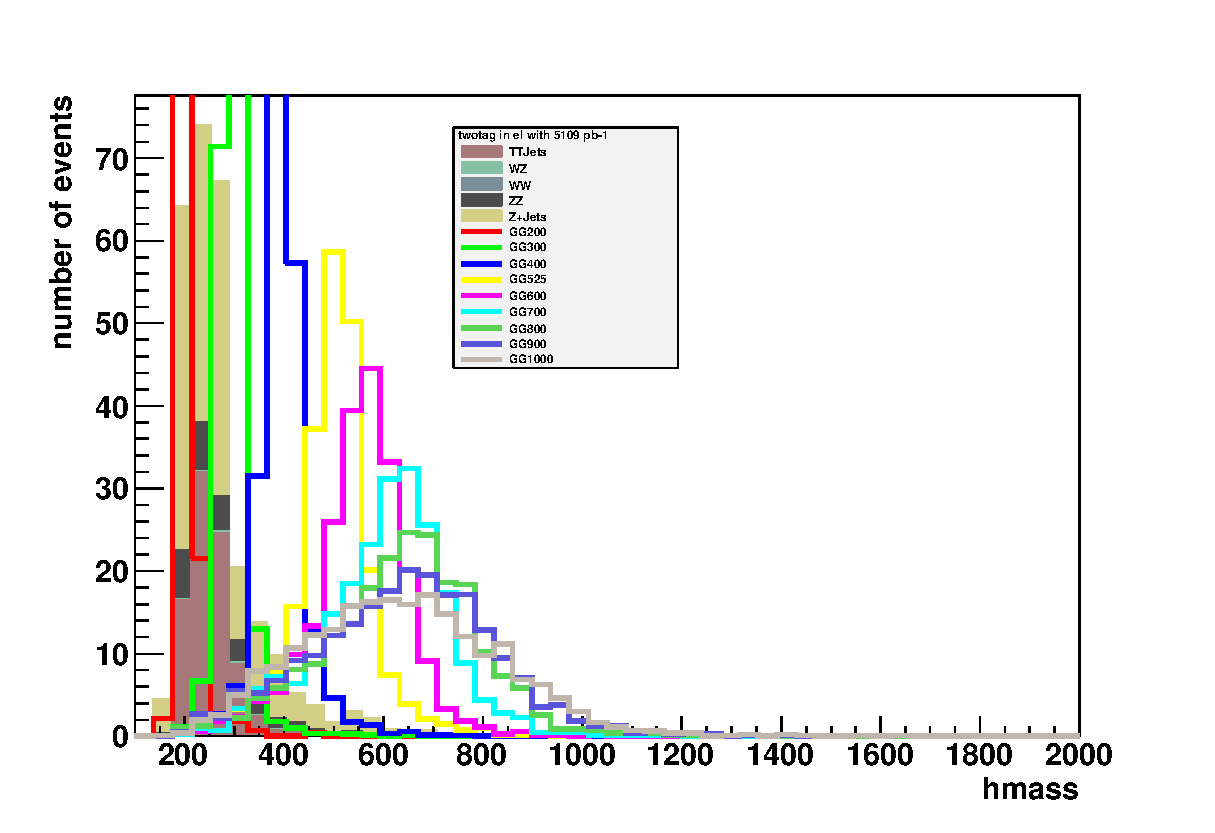
\includegraphics[width=0.5\textwidth]{images/mva_highmass/full_hmass.eps}
%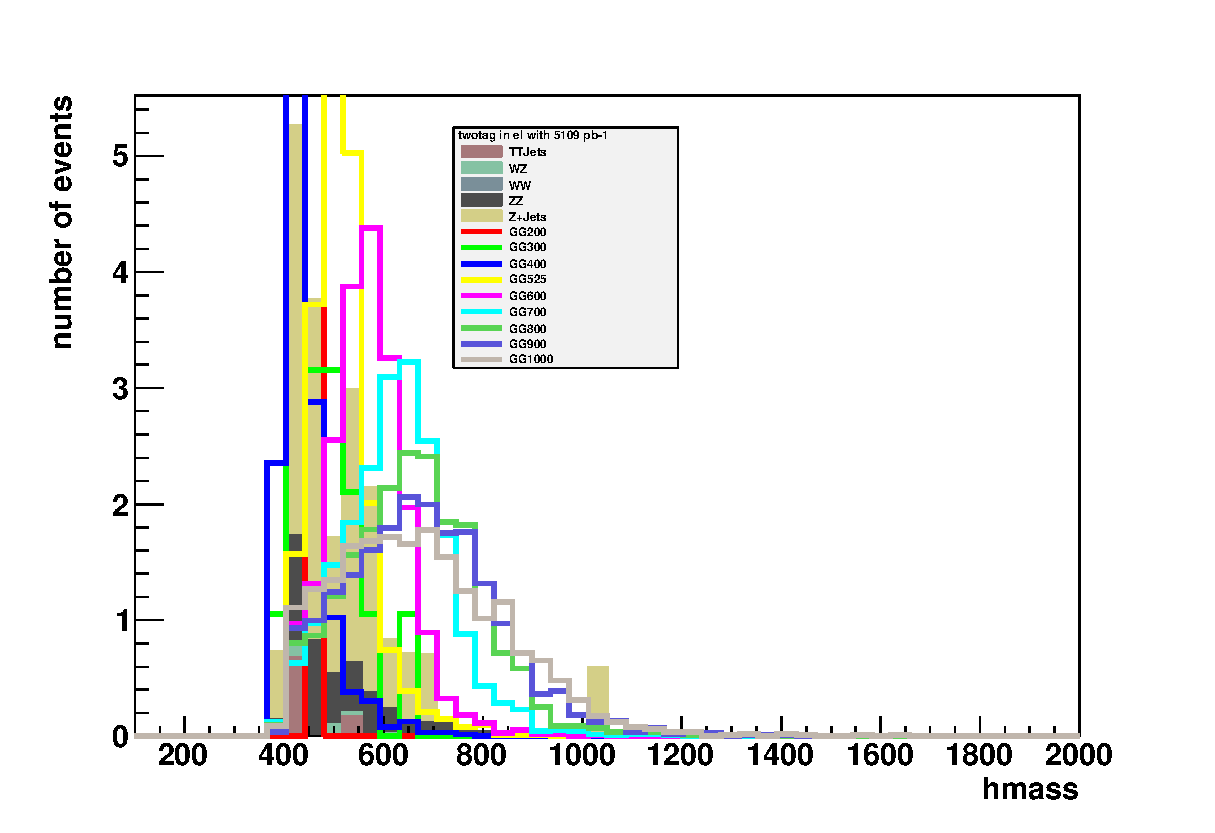
\includegraphics[width=0.5\textwidth]{images/mva_highmass/hmass.eps}\\
%  Twotag region Electrons (signal normalized to background)
%\end{center}
%\end{frame}

\begin{frame}{MLP}
\begin{center}
Electrons (zero,one,two)\\
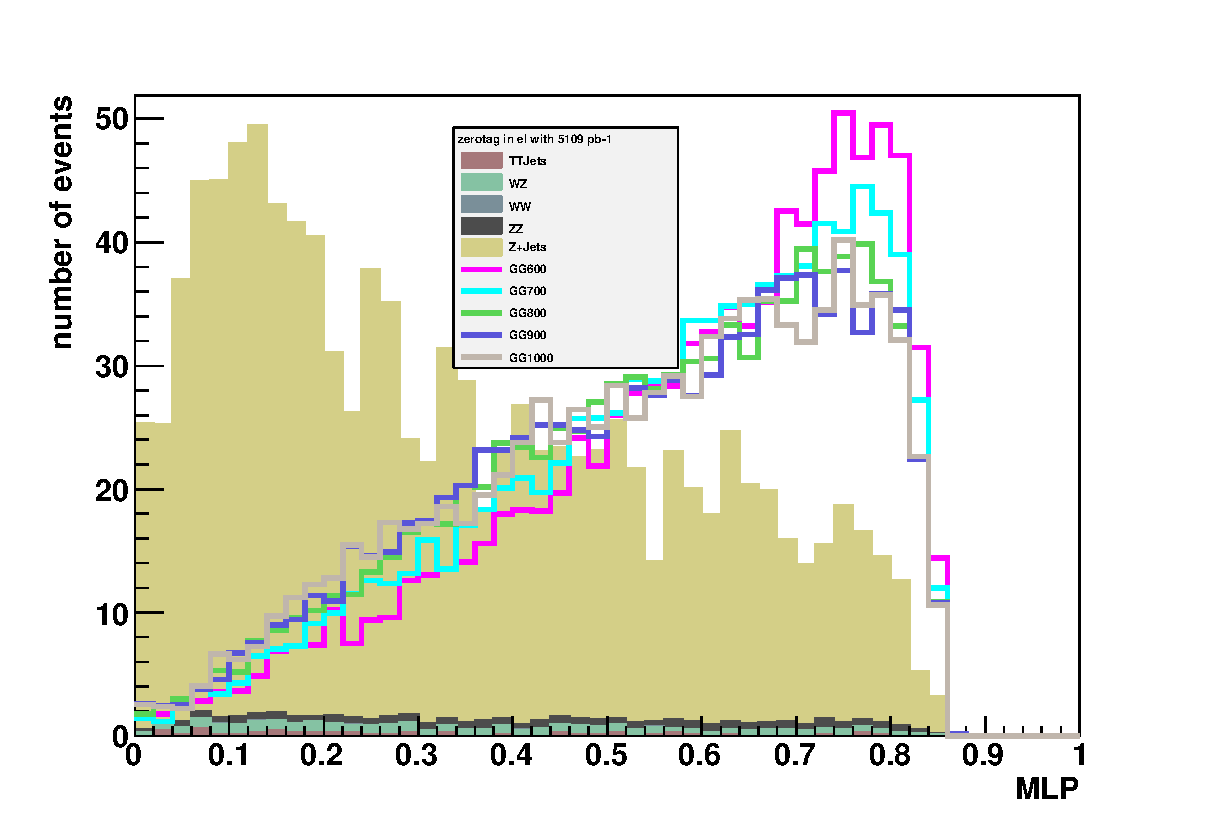
\includegraphics[width=0.33\textwidth]{images/mva_highmass/zero_MLP.eps}
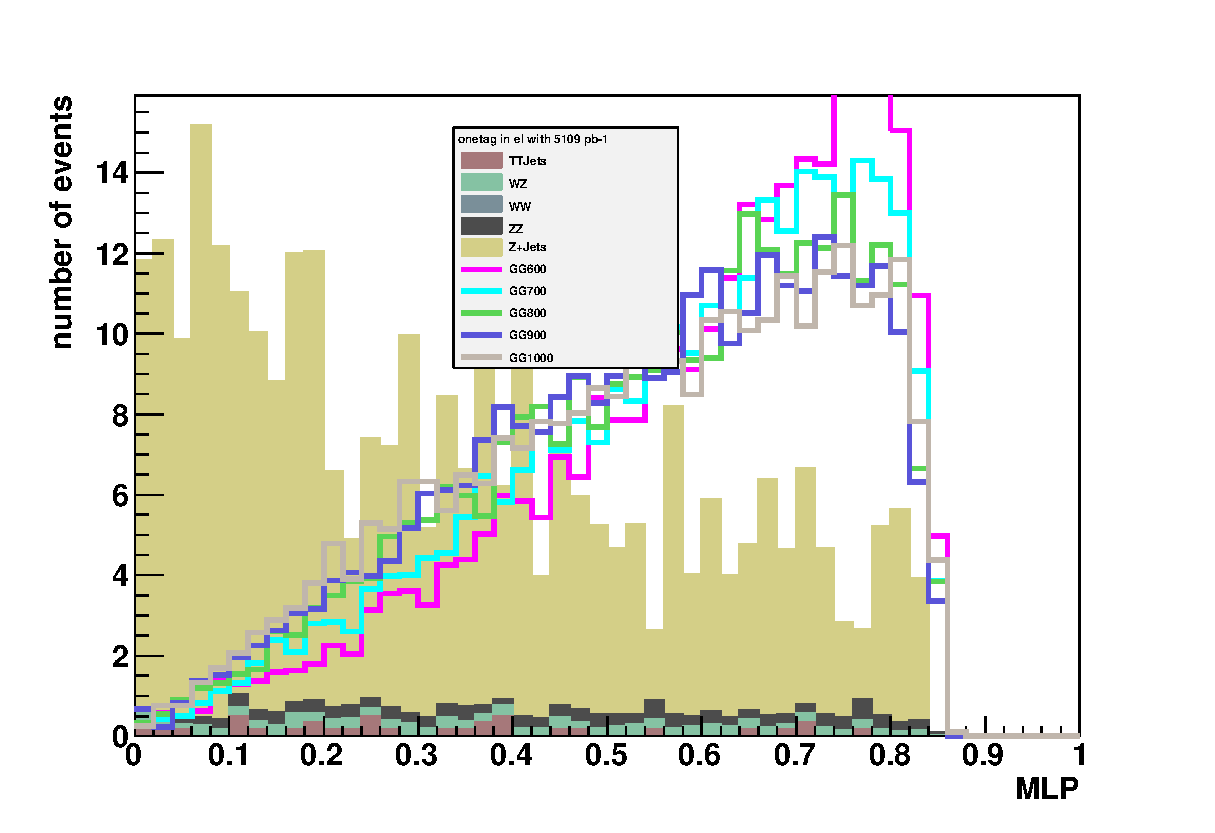
\includegraphics[width=0.33\textwidth]{images/mva_highmass/one_MLP.eps}
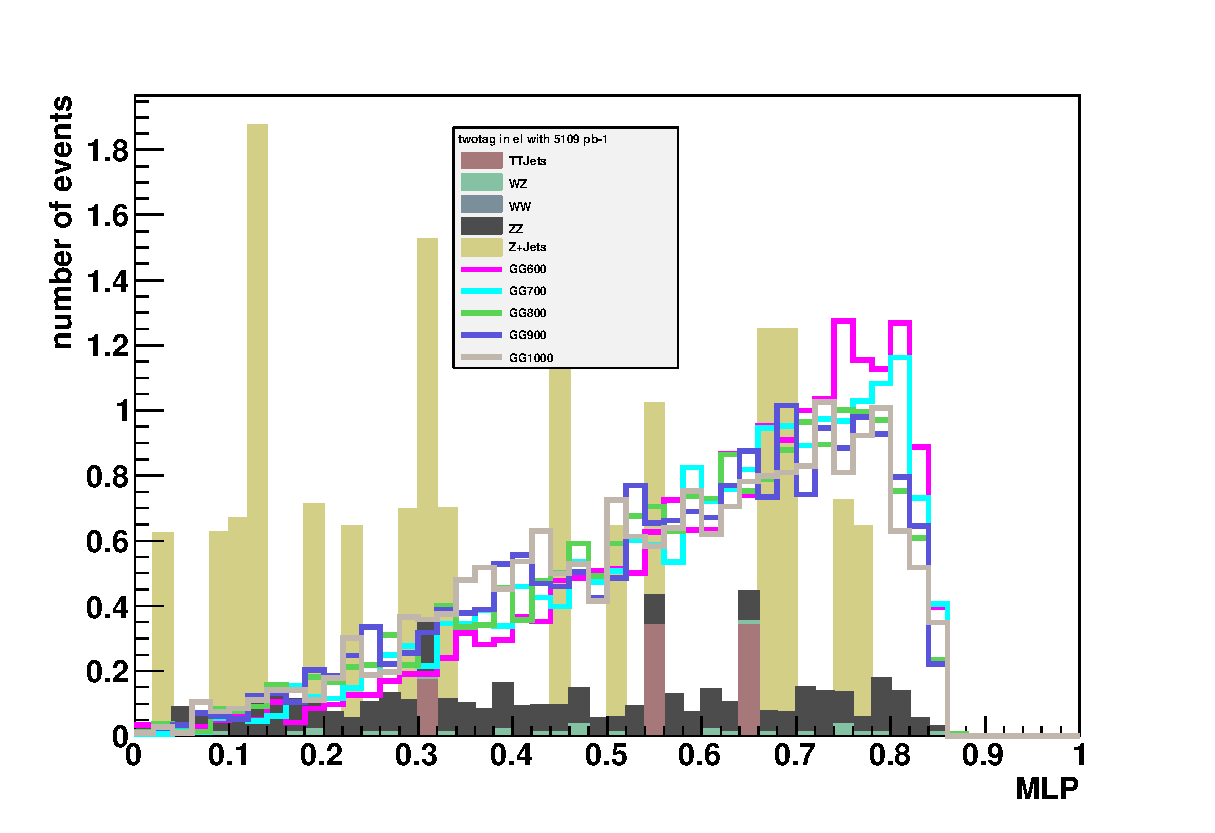
\includegraphics[width=0.33\textwidth]{images/mva_highmass/two_MLP.eps}\\
Muons (zero,one,two)\\
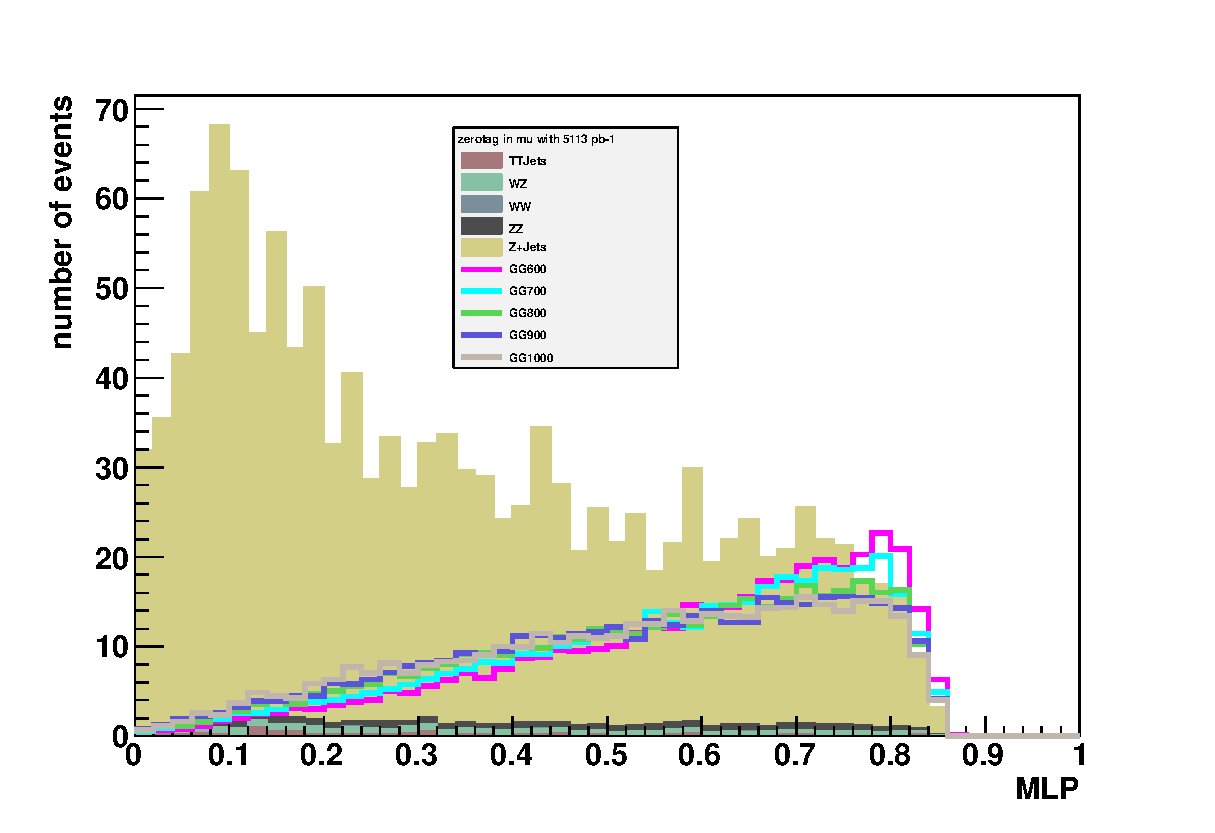
\includegraphics[width=0.33\textwidth]{images/mva_highmass/zero_mu_MLP.eps}
\includegraphics[width=0.33\textwidth]{images/mva_highmass/one_mu_MLP.eps}
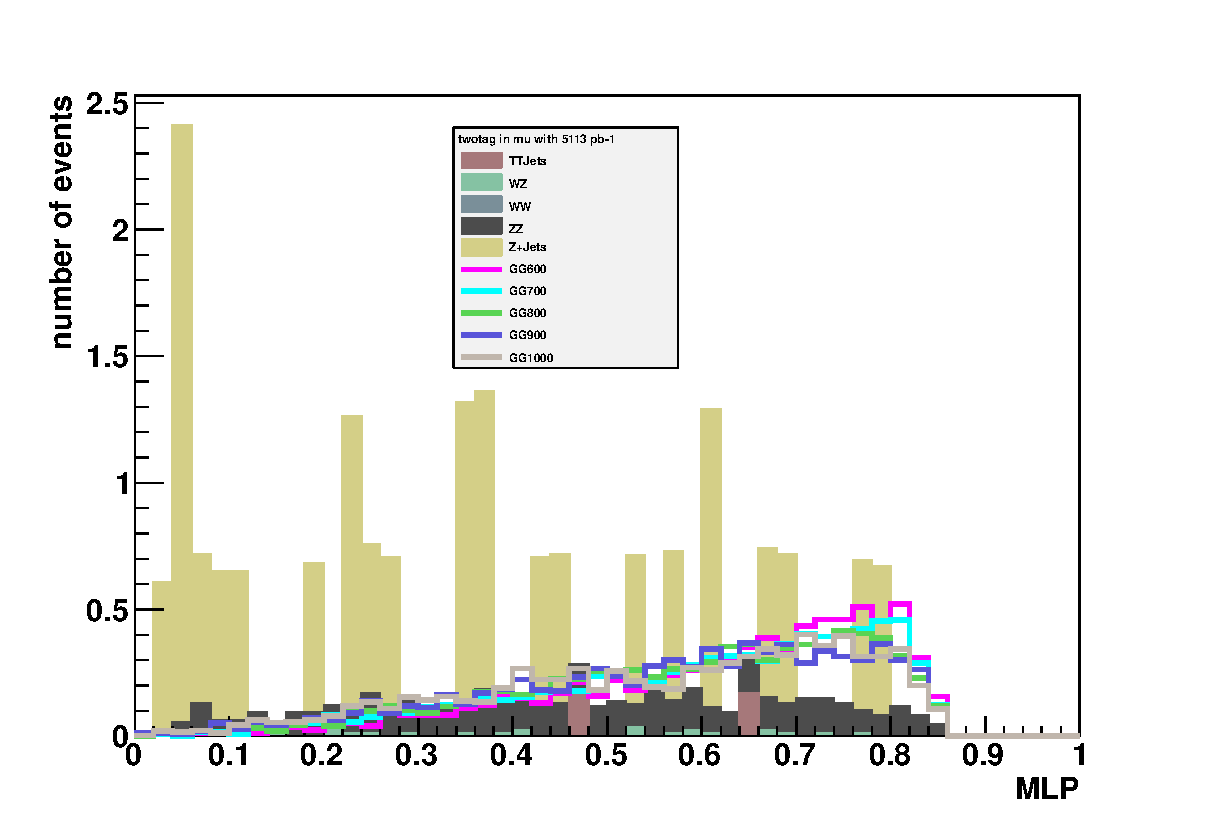
\includegraphics[width=0.33\textwidth]{images/mva_highmass/two_mu_MLP.eps}\\
\end{center}
\end{frame}



